\documentclass[a4paper]{article}

% \usepackage[utf8]{inputenc}
% \usepackage[T1]{fontenc}
% \usepackage{textcomp}
% \usepackage[english]{babel}
\usepackage{amsmath, amssymb}
\usepackage[marginparwidth=1.75cm]{geometry}
\usepackage{subfig}
\usepackage[colorlinks=true, anchorcolor=blue, linkcolor=blue, citecolor=blue, bookmarks=false,hyperfootnotes=false]{hyperref}
\usepackage{longtable}
\usepackage{siunitx}

\usepackage{verbatim}

% figure support
\usepackage{import}
\usepackage{xifthen}
\pdfminorversion=7
\usepackage{pdfpages}
\usepackage{transparent}
\usepackage{graphicx}
\newcommand{\incfig}[1]{%
		\def\svgwidth{\columnwidth}
		\import{./figures/}{#1.pdf_tex}
}

\graphicspath{ {./data/} }

\pdfsuppresswarningpagegroup=1

\begin{document}
\title{A249: Laser Gyroscope}
\maketitle 

In here we will present the tasks that we have to complete before conducting the lab. 

\section{Getting Started with Gyroscopes} \label{sec:getting_started}

We downloaded the \texttt{phyphox} app made by RWTH Aachen University, and we played around with the Gyroscope function. We rotated the phone in several directions 
to observe the relationship between the orientation of the phone and the corresponding coordinates used in the application. This is shown in Fig. \ref{fig:phone_sketch}. 
Fig. \ref{fig:gyro_plot_z} - \ref{fig:gyro_plot_x} show the corresponding time series for the $x, y, z$ coordinates for each rotation that we performed. 

\begin{figure*}[hbt!]
	\centering
	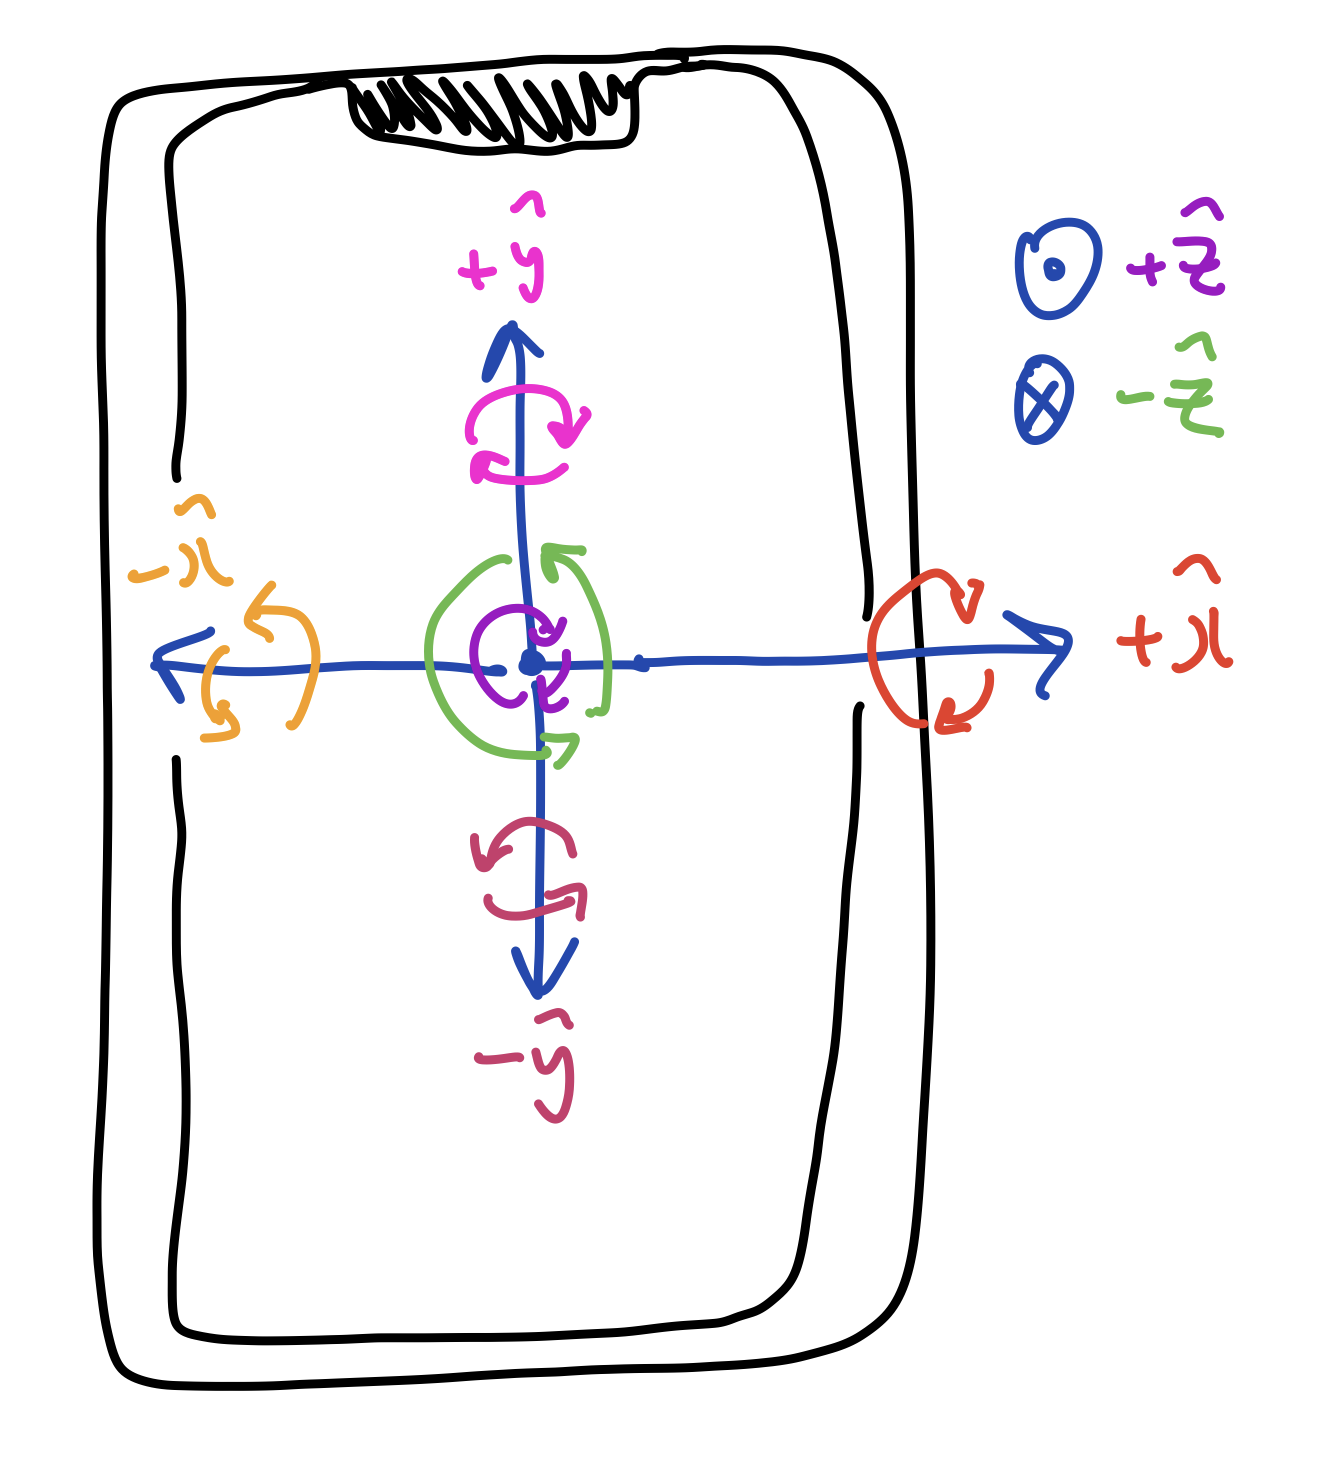
\includegraphics[width=0.6\columnwidth]{Phone_sketch.png}

	\caption{Sketch of the phone used to measure the gyroscope with its relevant $x, y, z$ coordinates and sense of rotation. 
            The sense of rotation is color coded with each rotation axis, and the direction of the axis is indicated by the blue arrows.}
	\label{fig:phone_sketch}
\end{figure*}

\begin{figure*}[hbt!]
	\centering
	\subfloat[$+z$ direction, anti-clockwise]{{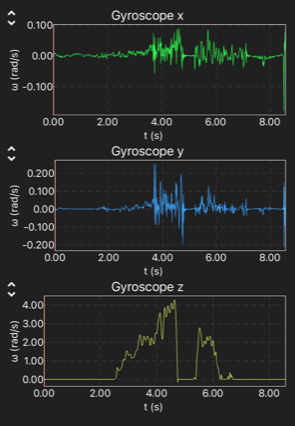
\includegraphics[width=0.3\columnwidth]{rotation_posz.PNG}}}
	\quad
	\subfloat[$-z$ direction, clockwise]{{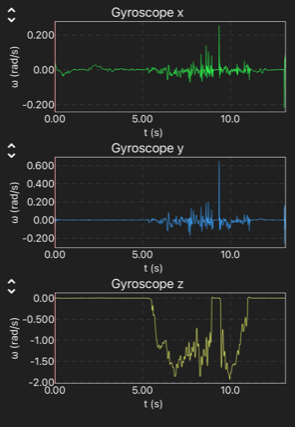
\includegraphics[width=0.3\columnwidth]{rotation_negz.PNG}}}

	\caption{The time series of the $x, y, z$ coordinates shown from the \texttt{phyphox} application when 
            the phone was rotated parallel to the surface. This corresponds to rotations in the $z$-direction. Note the large amplitudes in 
            the time series, which indicates rotations in the relevant axis. }
	\label{fig:gyro_plot_z}
\end{figure*}


\begin{figure*}[hbt!]
	\centering
	\subfloat[$+y$ direction, into surface (anti-clockwise)]{{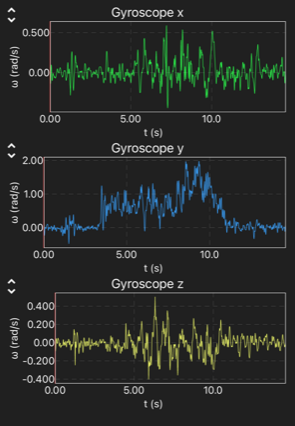
\includegraphics[width=0.3\columnwidth]{rotation_posy.PNG}}}
	\quad
	\subfloat[$-y$ direction, out of surface (clockwise)]{{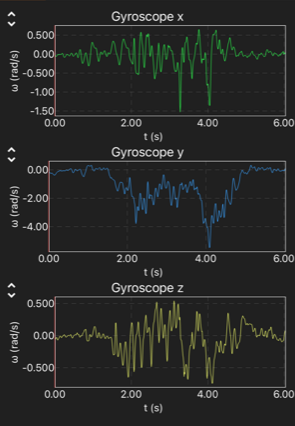
\includegraphics[width=0.3\columnwidth]{rotation_negy.PNG}}}

	\caption{Same as Fig. \ref{fig:gyro_plot_z} but for rotations into / out of the surface, corresponding to rotations in $y$-direction.}
	\label{fig:gyro_plot_y}
\end{figure*}


\begin{figure*}[hbt!]
	\centering
	\subfloat[$+x$ direction, rotation towards user (anti-clockwise)]{{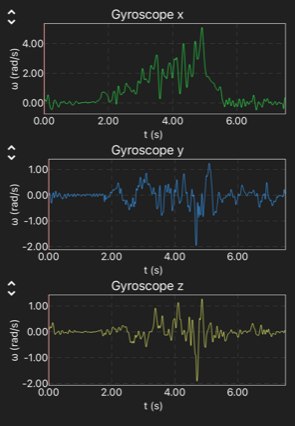
\includegraphics[width=0.3\columnwidth]{rotation_posx.PNG}}}
	\quad
	\subfloat[$-x$ direction, rotation away from user (clockwise)]{{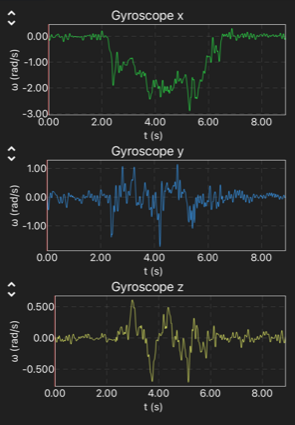
\includegraphics[width=0.3\columnwidth]{rotation_negx.PNG}}}

	\caption{Same as Fig. \ref{fig:gyro_plot_z} but for rotations towards / away the user, corresponding to rotations in $x$-direction.}
	\label{fig:gyro_plot_x}
\end{figure*}

To save the rotation rates and import it into the computer for further analysis, the \texttt{Export Data} feature can be utilized. This will save the 
data as a \texttt{.zip} file that contains the raw data, the software and specifics regarding the device used, and the system time in which the experiment was 
started and finished. All such files are saved as \texttt{.csv} formats. An example for the raw data is shown in the Appendix section.\par 

To obtain a faster rotation rate, we applied maximal torque on each end of the phone such that the rotation at each axis was maximal. This was done at an adequate height
to ensure the rotation rate was properly measured. Several cushions were placed on top of a bed to ensure that the phone does not break. Fig. \ref{fig:gyro_plot_fast} show
the time series of the $x, y, z$ coordinates in the $+y$ and $-z$ directions. Performing the measurement in such a way yields a more notable and stable measurement of the rotation rate 

\begin{figure*}[hbt!]
	\centering
	\subfloat[$+y$ direction \label{fig:gyro_plot_fast_y}]{{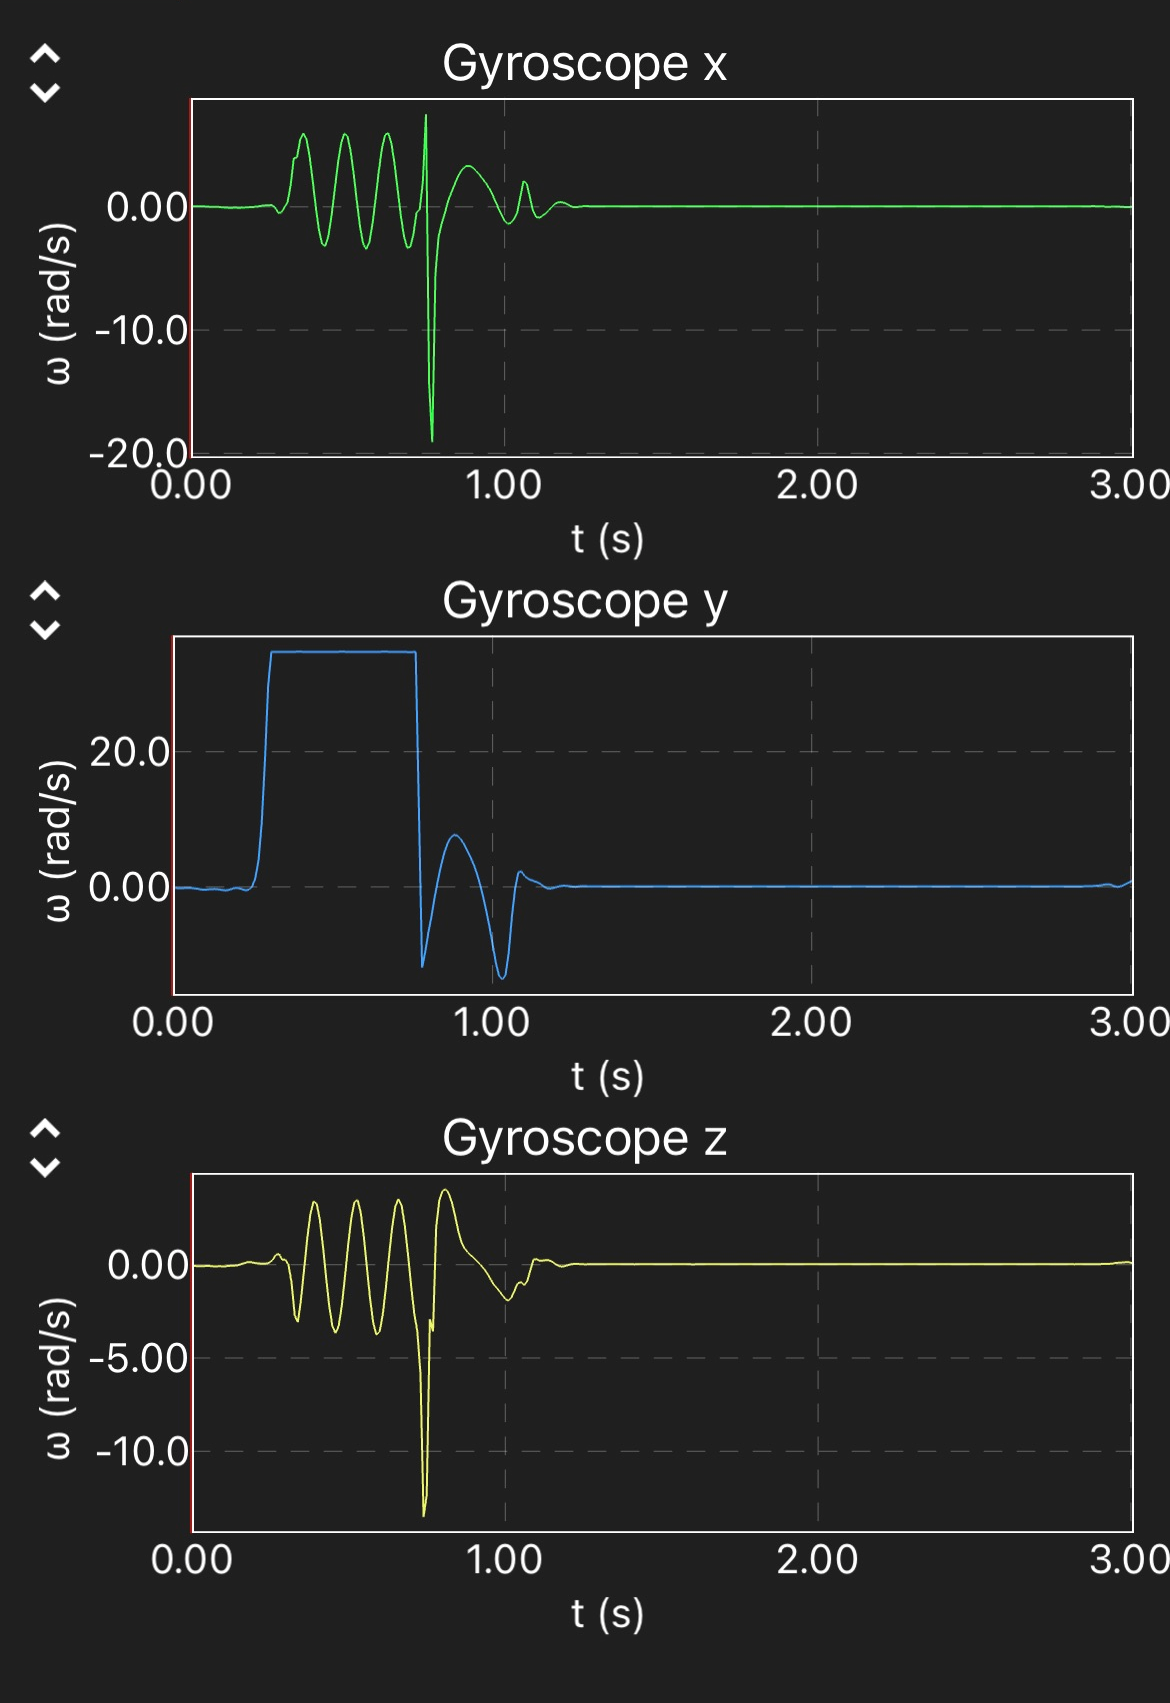
\includegraphics[width=0.3\columnwidth]{rot_fast_posy.png}}}
	\quad
	\subfloat[$-z$ direction \label{fig:gyro_plot_fast_z}]{{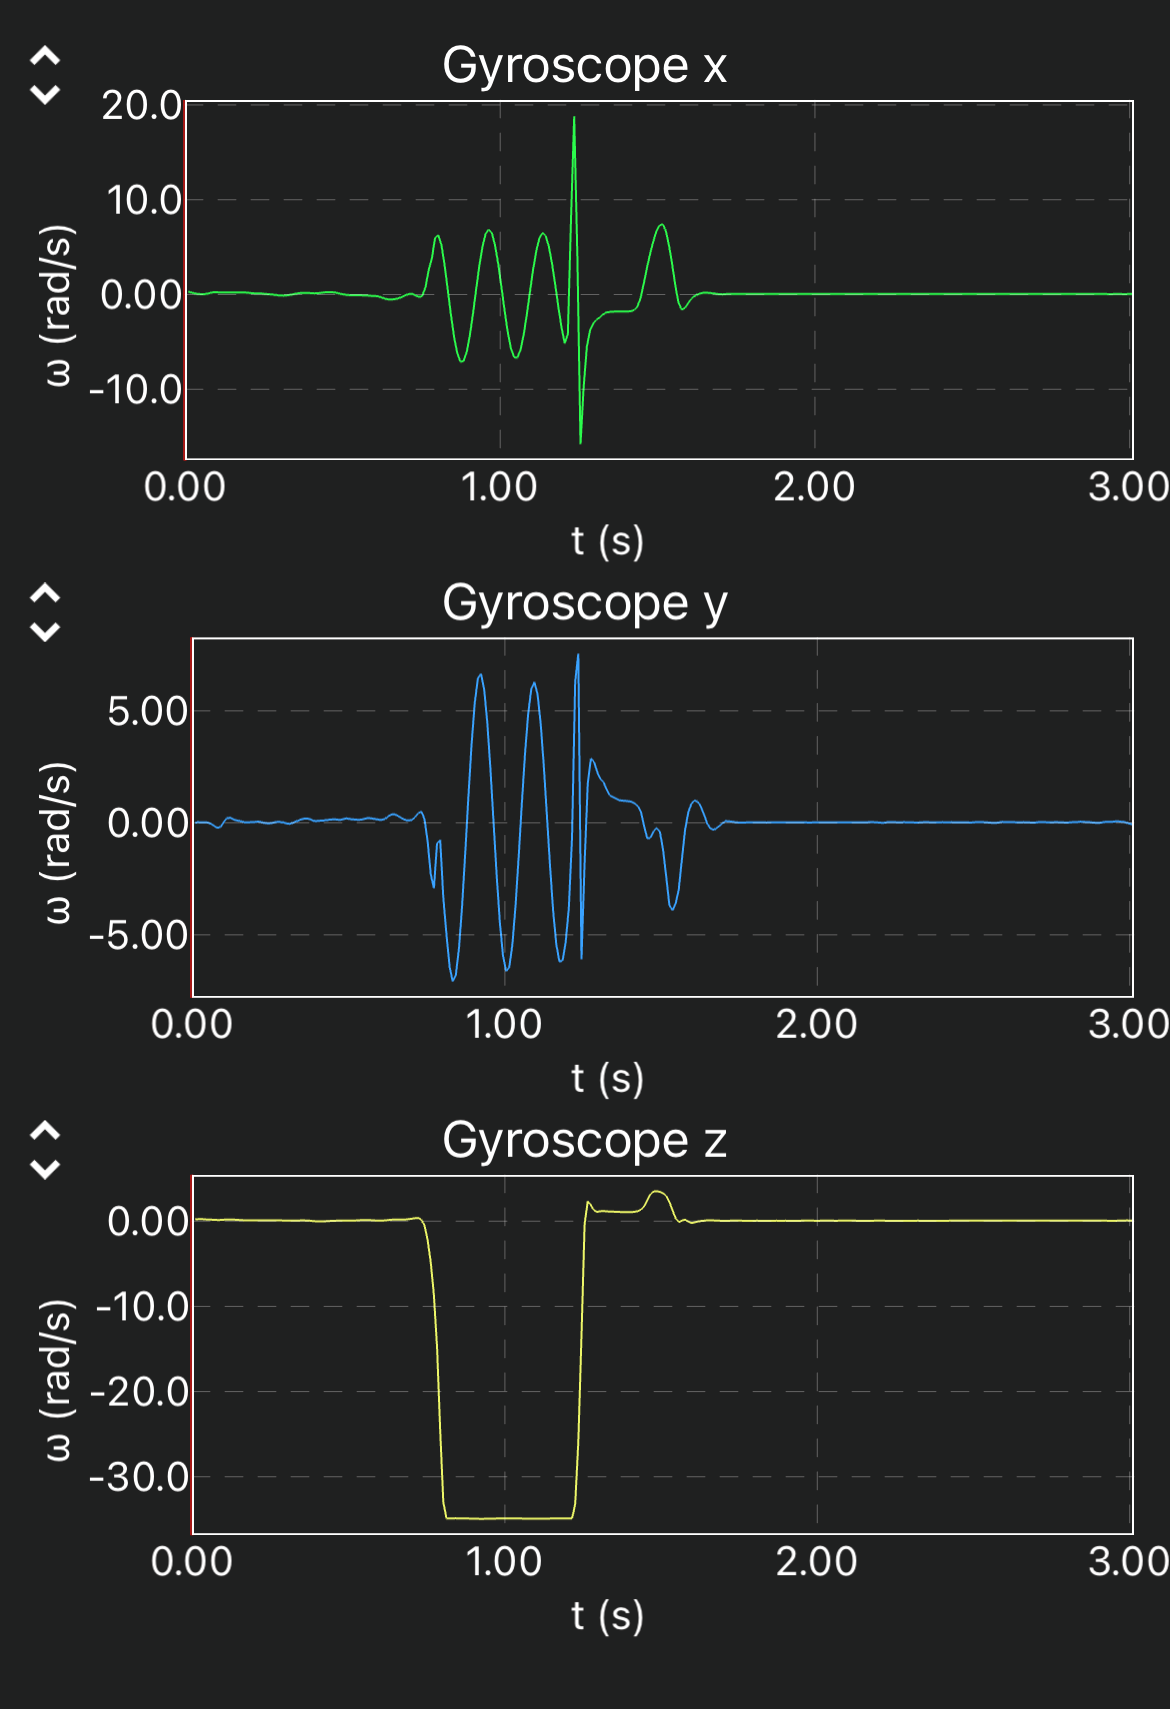
\includegraphics[width=0.3\columnwidth]{rot_fast_negz.PNG}}}

	\caption{Same as Fig. \ref{fig:gyro_plot_z} but for fast rotations in the (a) $+y$ and (b) $-z$ direction.}
	\label{fig:gyro_plot_fast}
\end{figure*}


\section{Allan Deviation}
We start off by keeping the phone flat on the ground for the duration of an hour and record the accelerometer of the phone. In Fig. \ref{fig:raw}, we see the raw data for individual axis of rotation. 

\begin{figure}[hbt!]
     \centering
	 {{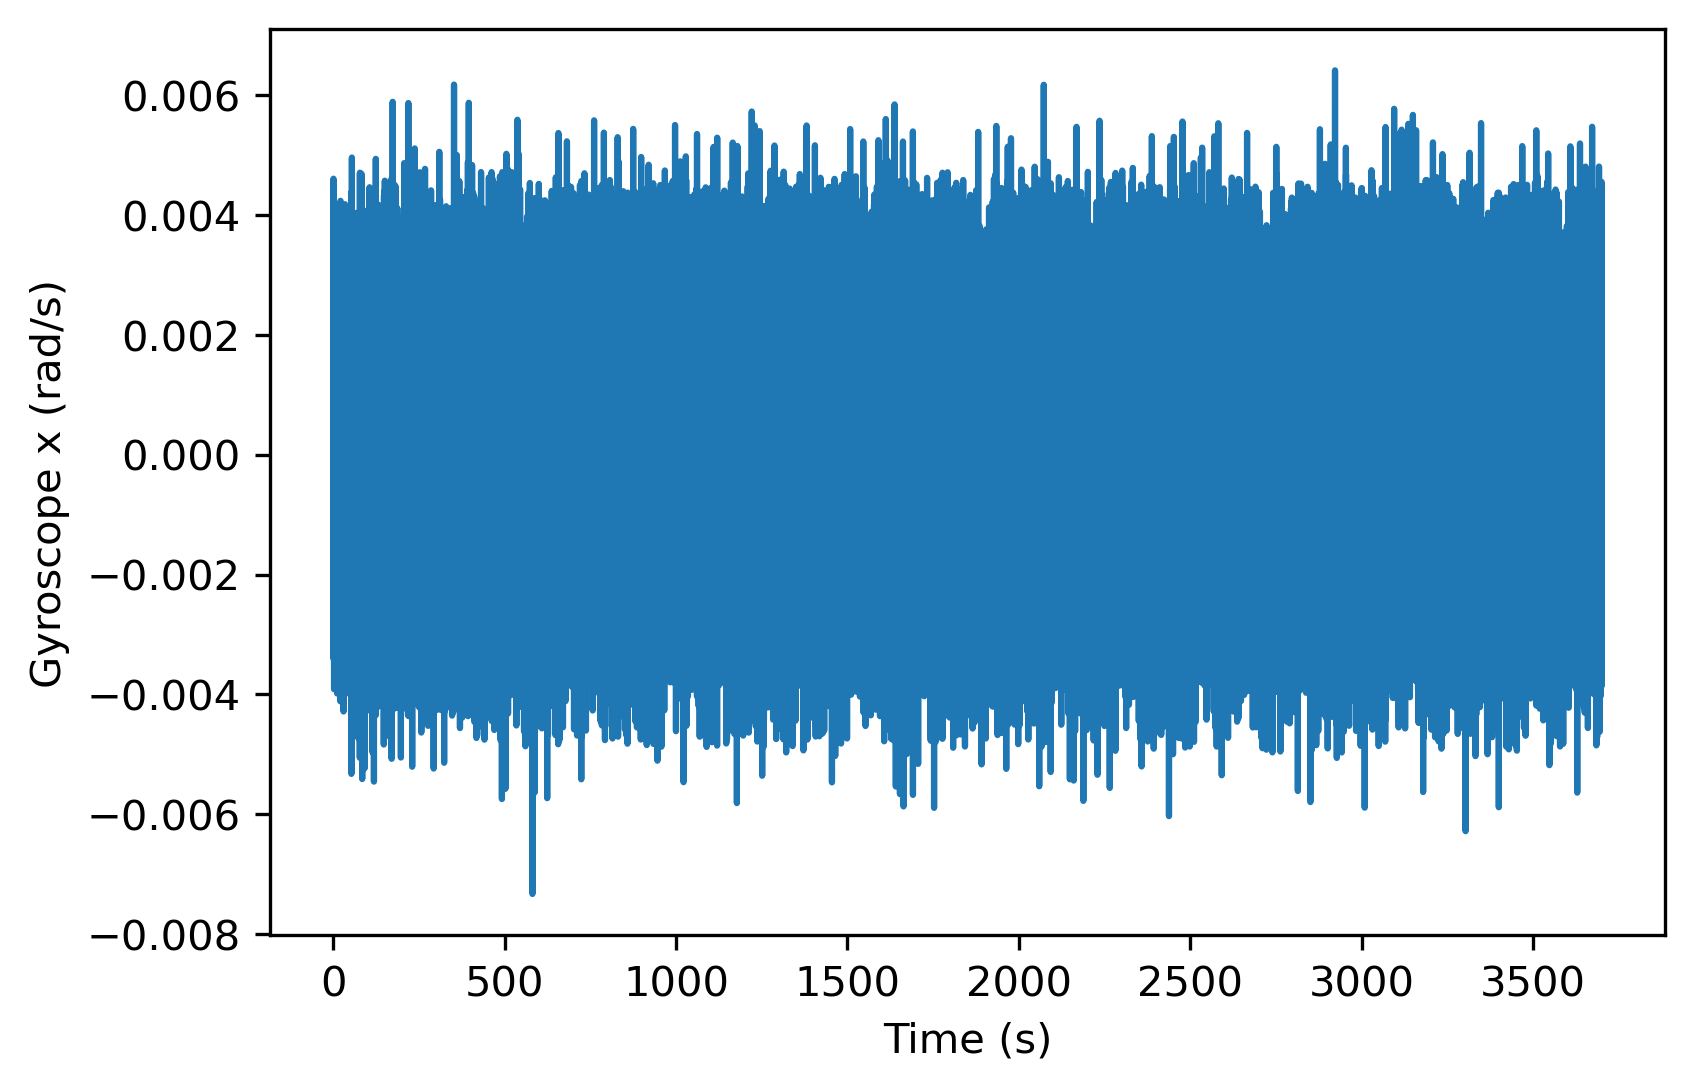
\includegraphics[width=0.4\columnwidth]{raw_x.png}}}
	 {{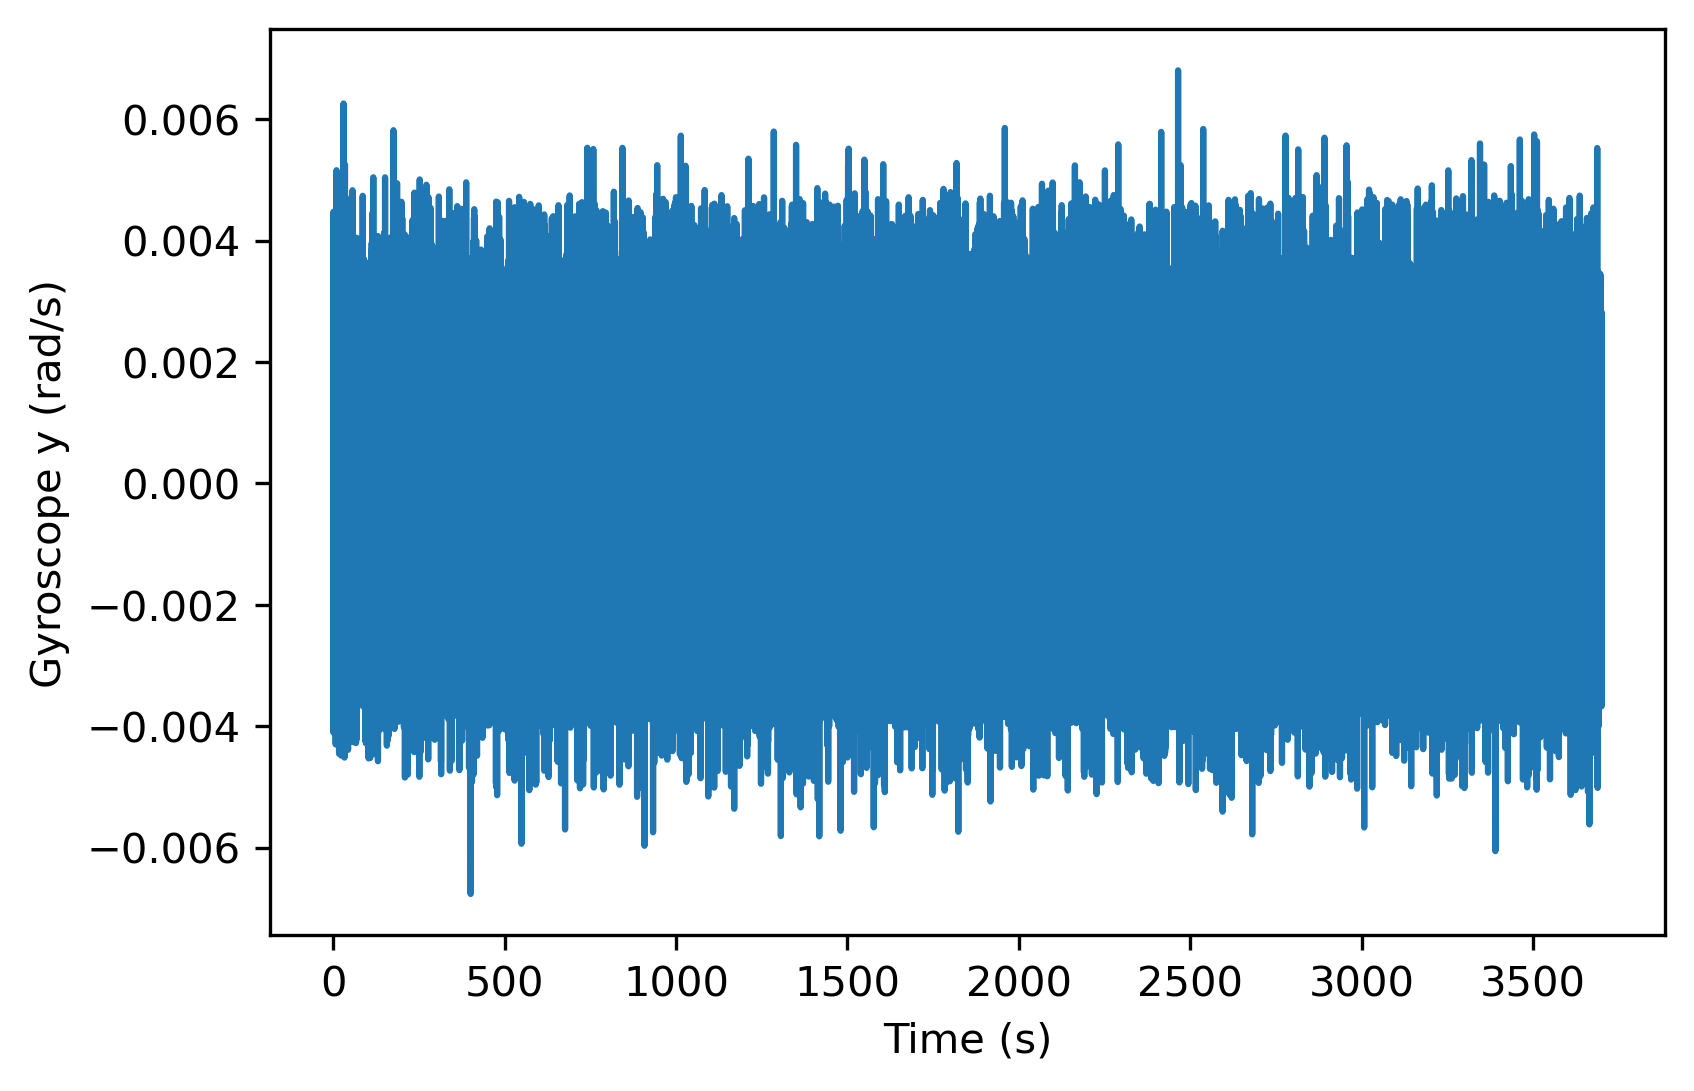
\includegraphics[width=0.4\columnwidth]{raw_y.png}}}
	 {{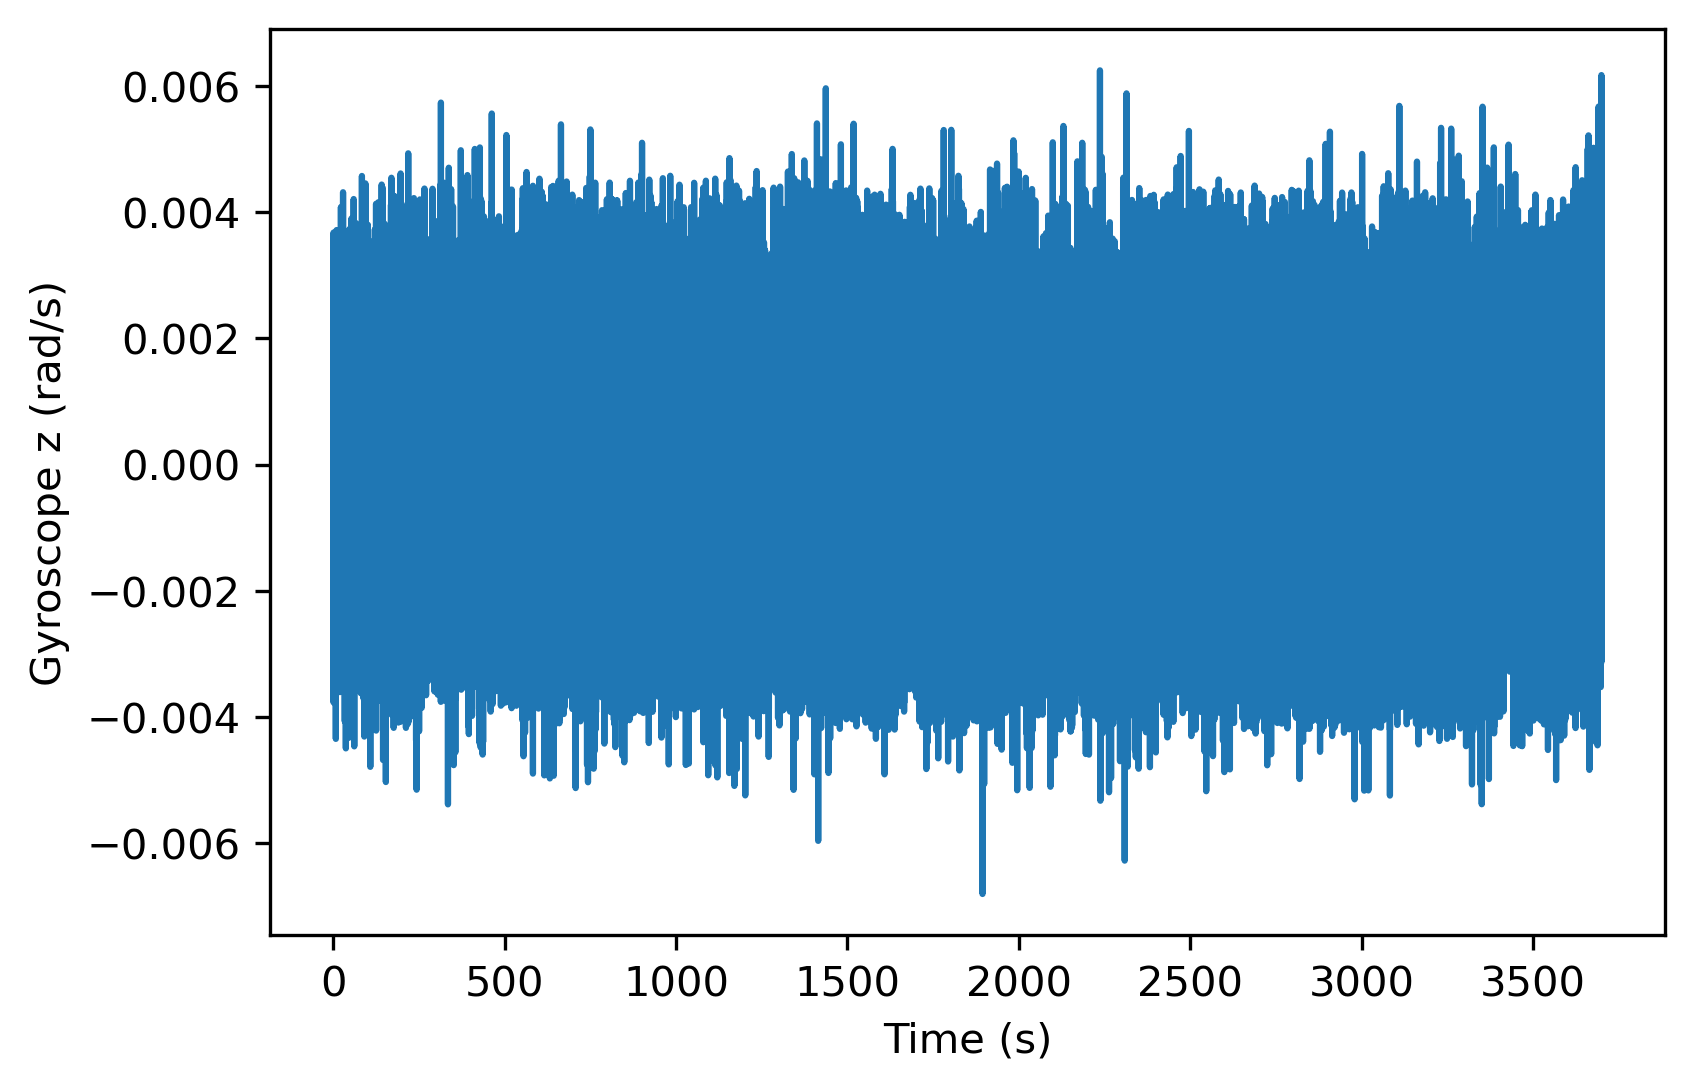
\includegraphics[width=0.4\columnwidth]{raw_z.png}}}
     \caption{Raw data of all the three axes of gyroscope from phone.}
	 \label{fig:raw}
\end{figure}

From these figures, it is difficult to come to any conclusion because all we see in random noise. To analyze it further, we will take the Fourier Transoform. For plotting the data in the frequency domain, we use the \texttt{numpy} tool from the \texttt{Python}. 

\begin{figure}[hbt!]
     \centering
	 {{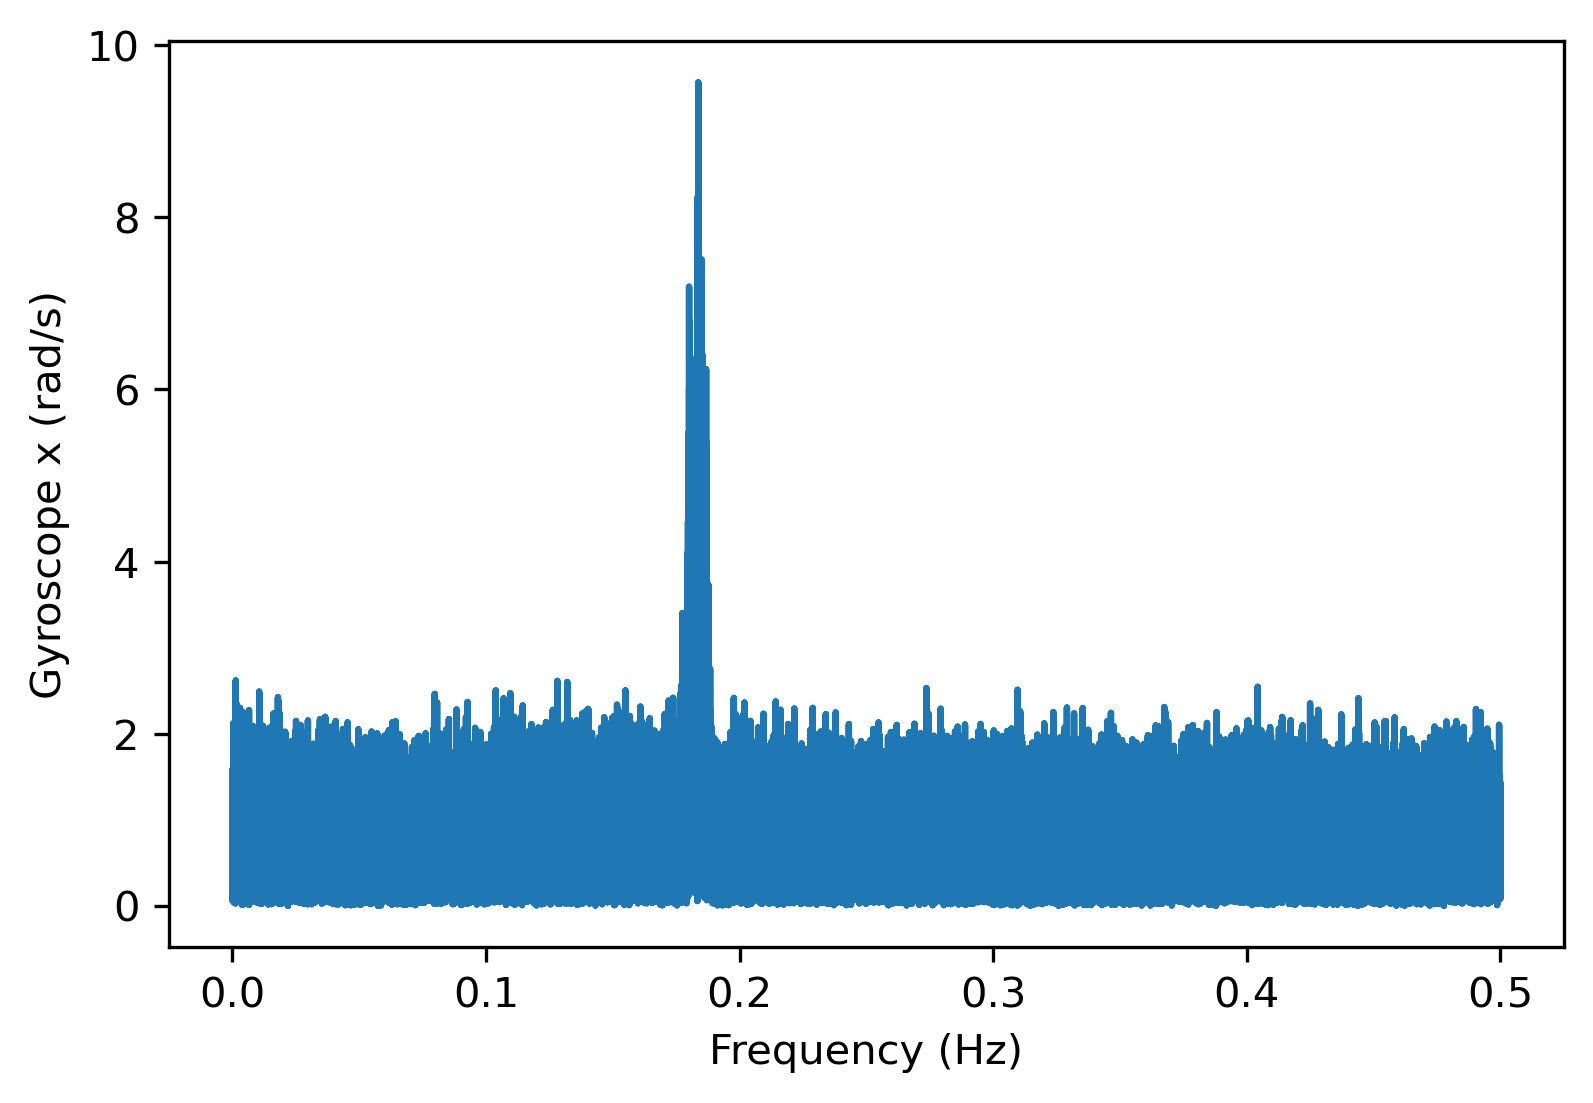
\includegraphics[width=0.4\columnwidth]{fft_x.png}}}
	 {{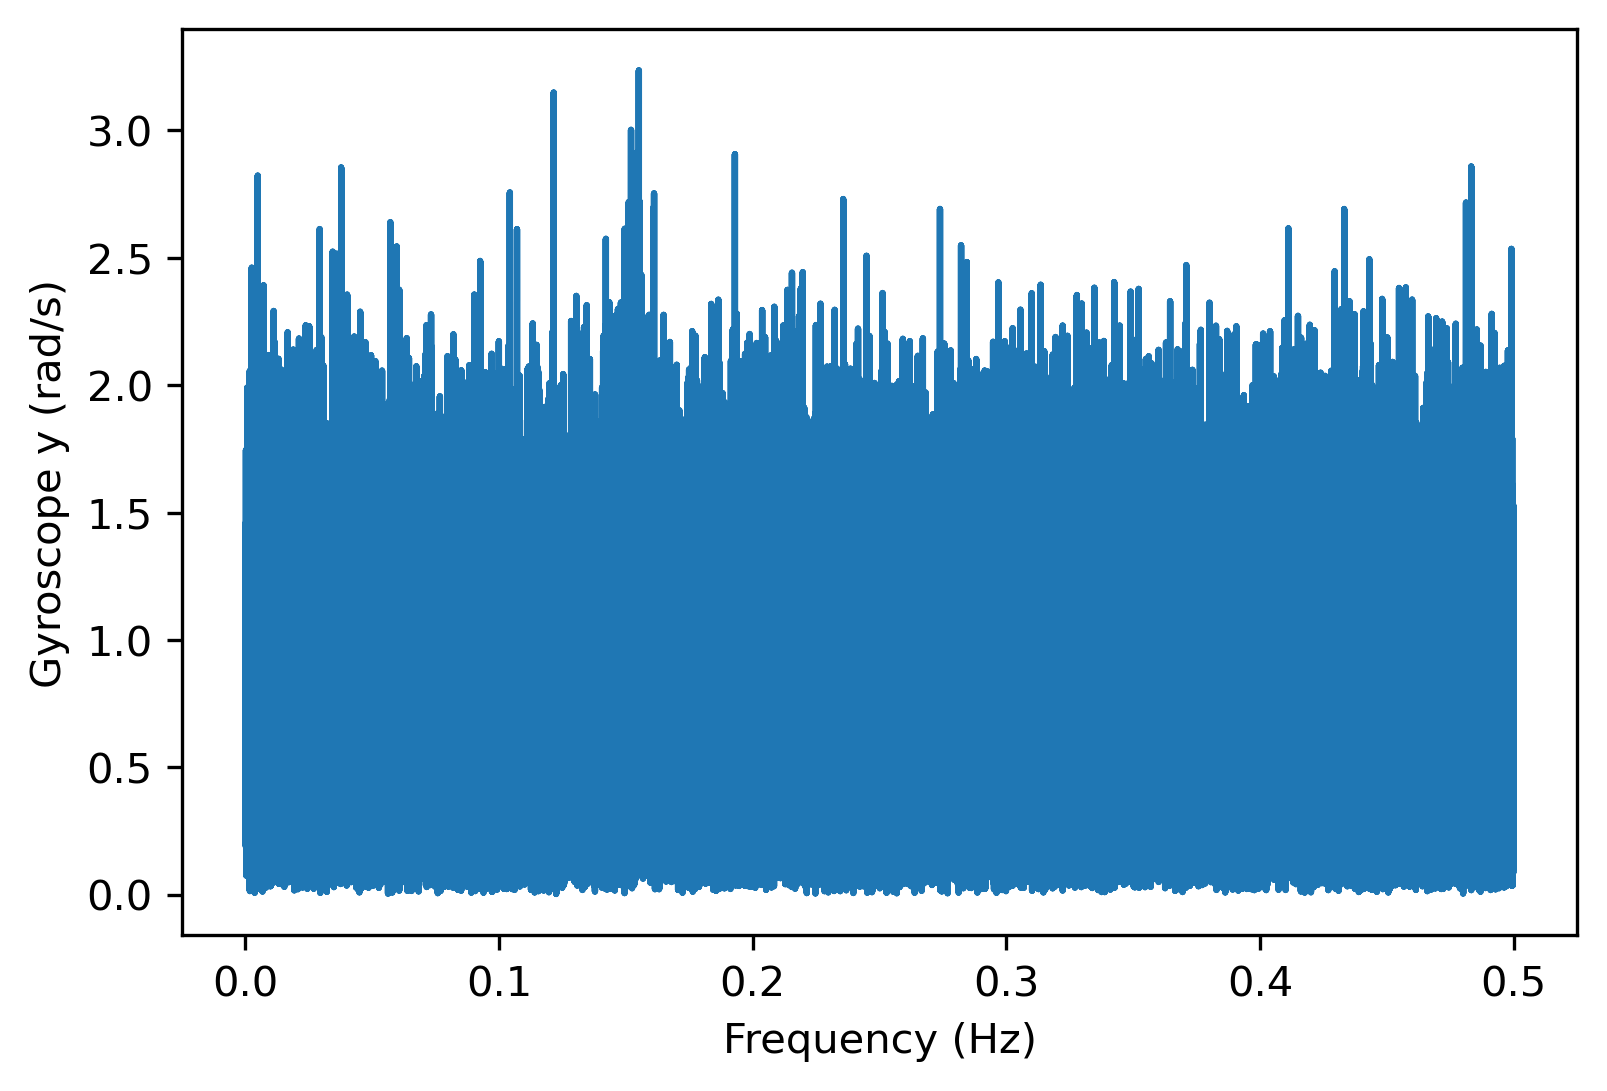
\includegraphics[width=0.4\columnwidth]{fft_y.png}}}
	 {{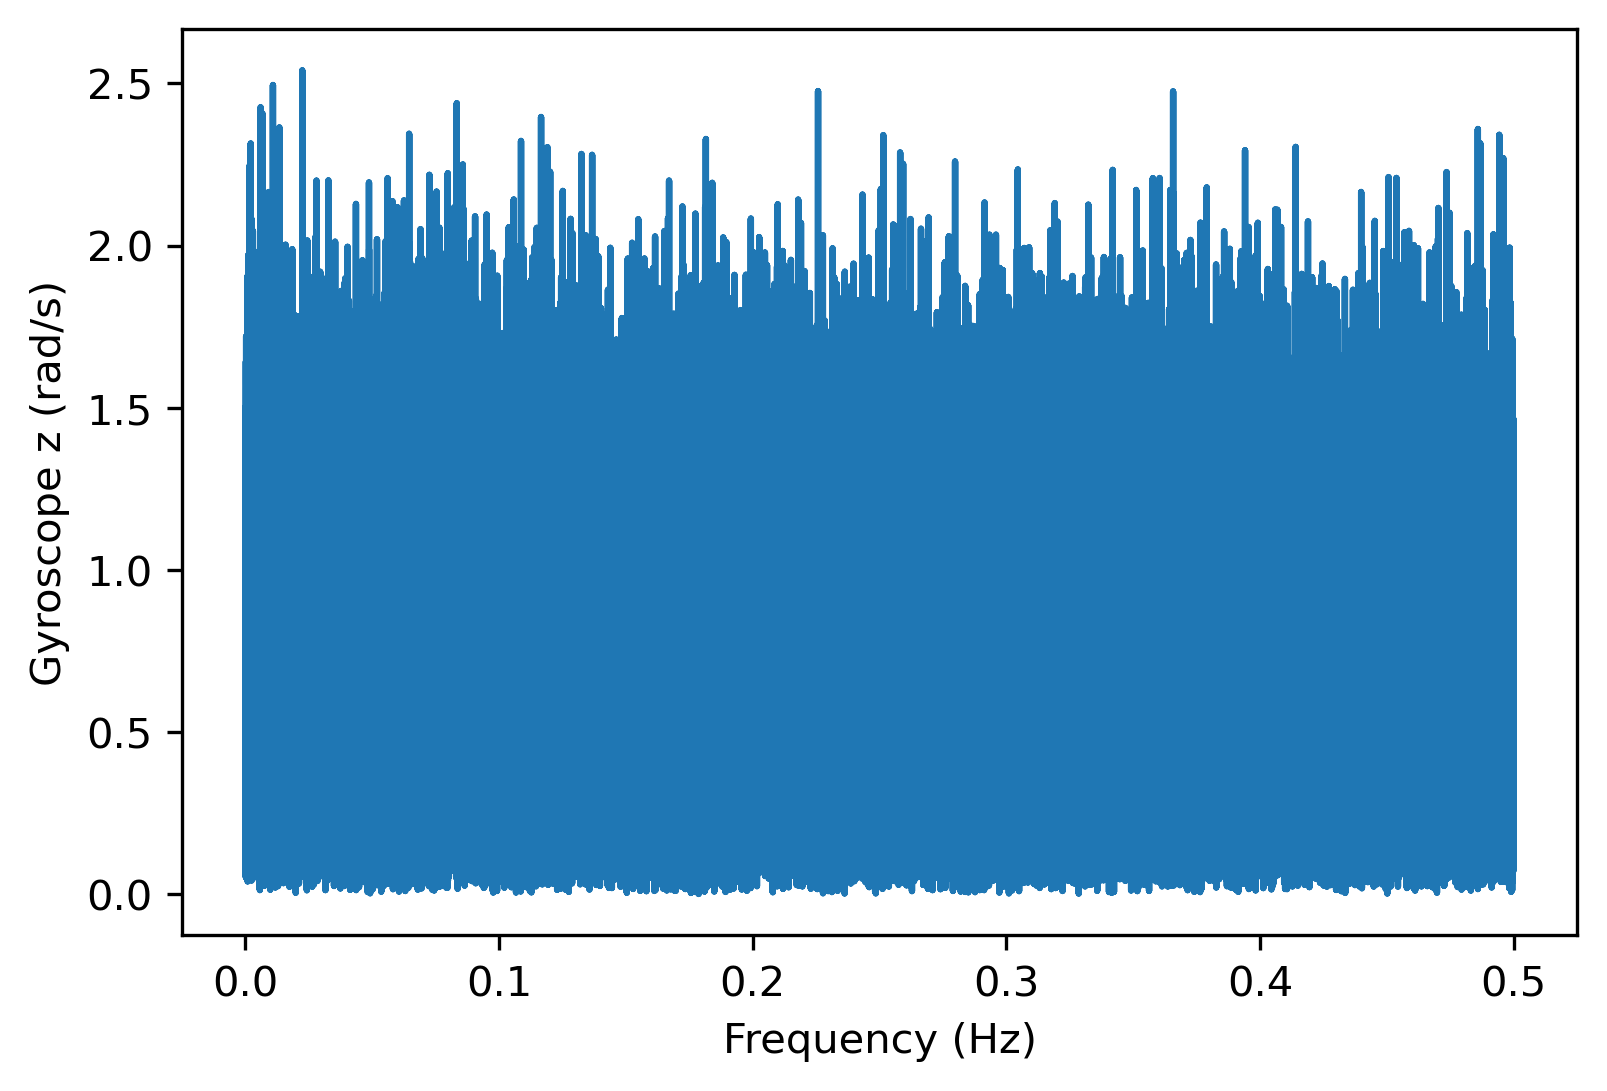
\includegraphics[width=0.4\columnwidth]{fft_z.png}}}
	 \caption{Fourier Transform of all 3 axes of the raw data.}
	 \label{fig:fft}
\end{figure}

In Fig. \ref{fig:fft}, we see that in the x-axis Fourier transform, there is a noticeable peak at approximately 0.19 Hz. This could be a small disturbance that might have been caused by some random movement. But it would have to be periodic enough to be noticeable. It also could be because of the rotation of earth but we would have to investigate this further. \\

For computing the Allan deviation for all of these plots, the function \texttt{adev()} was used from the Python package, \texttt{allantools}. 

\begin{figure}[hbt!]
     \centering
	 {{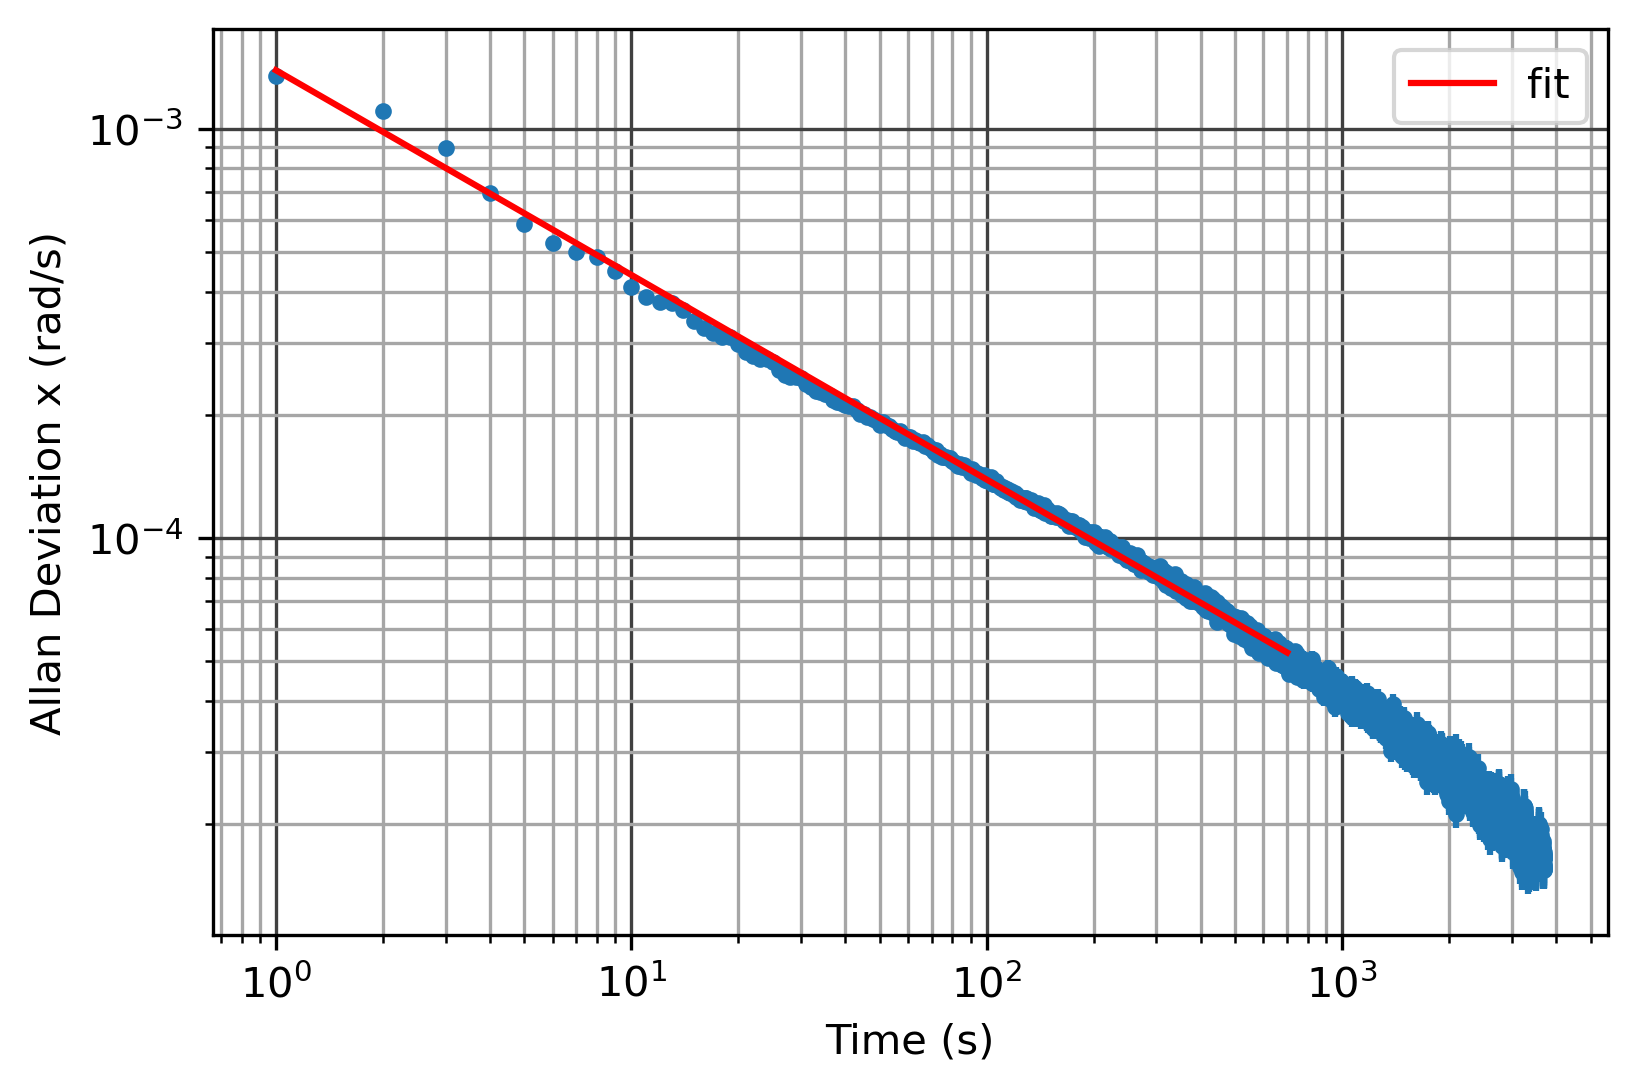
\includegraphics[width=0.4\columnwidth]{allan_x.png}}}
	 {{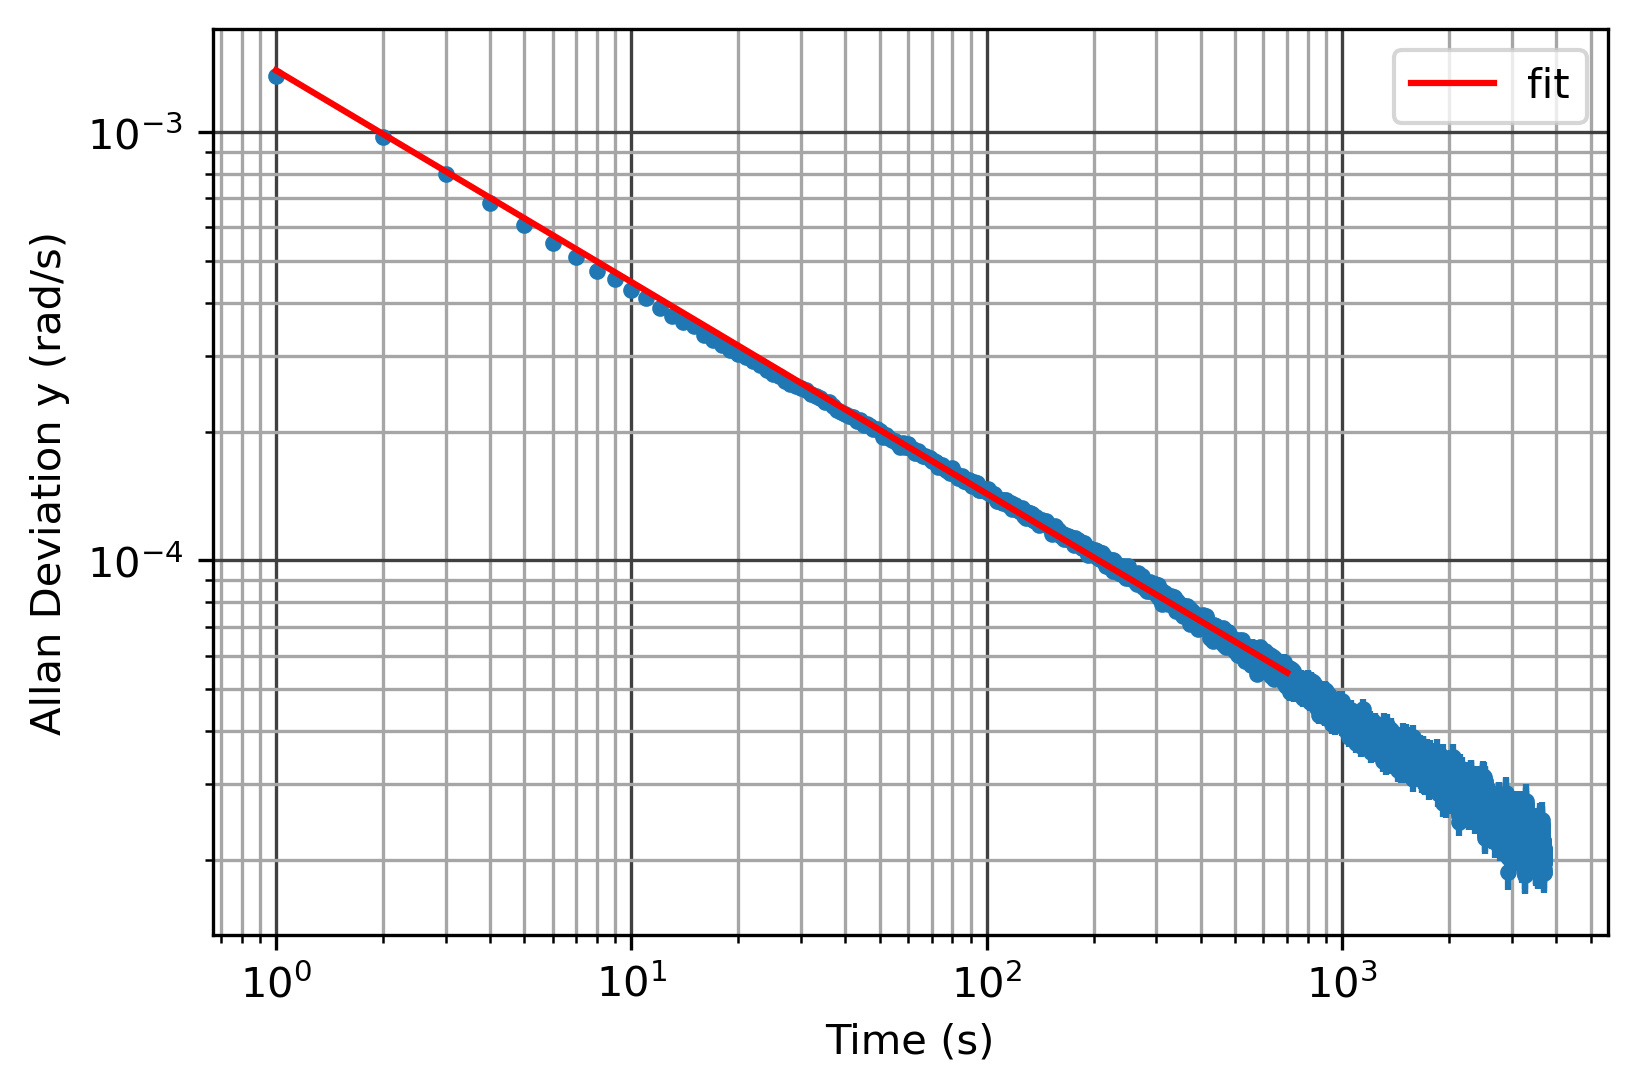
\includegraphics[width=0.4\columnwidth]{allan_y.png}}}
	 {{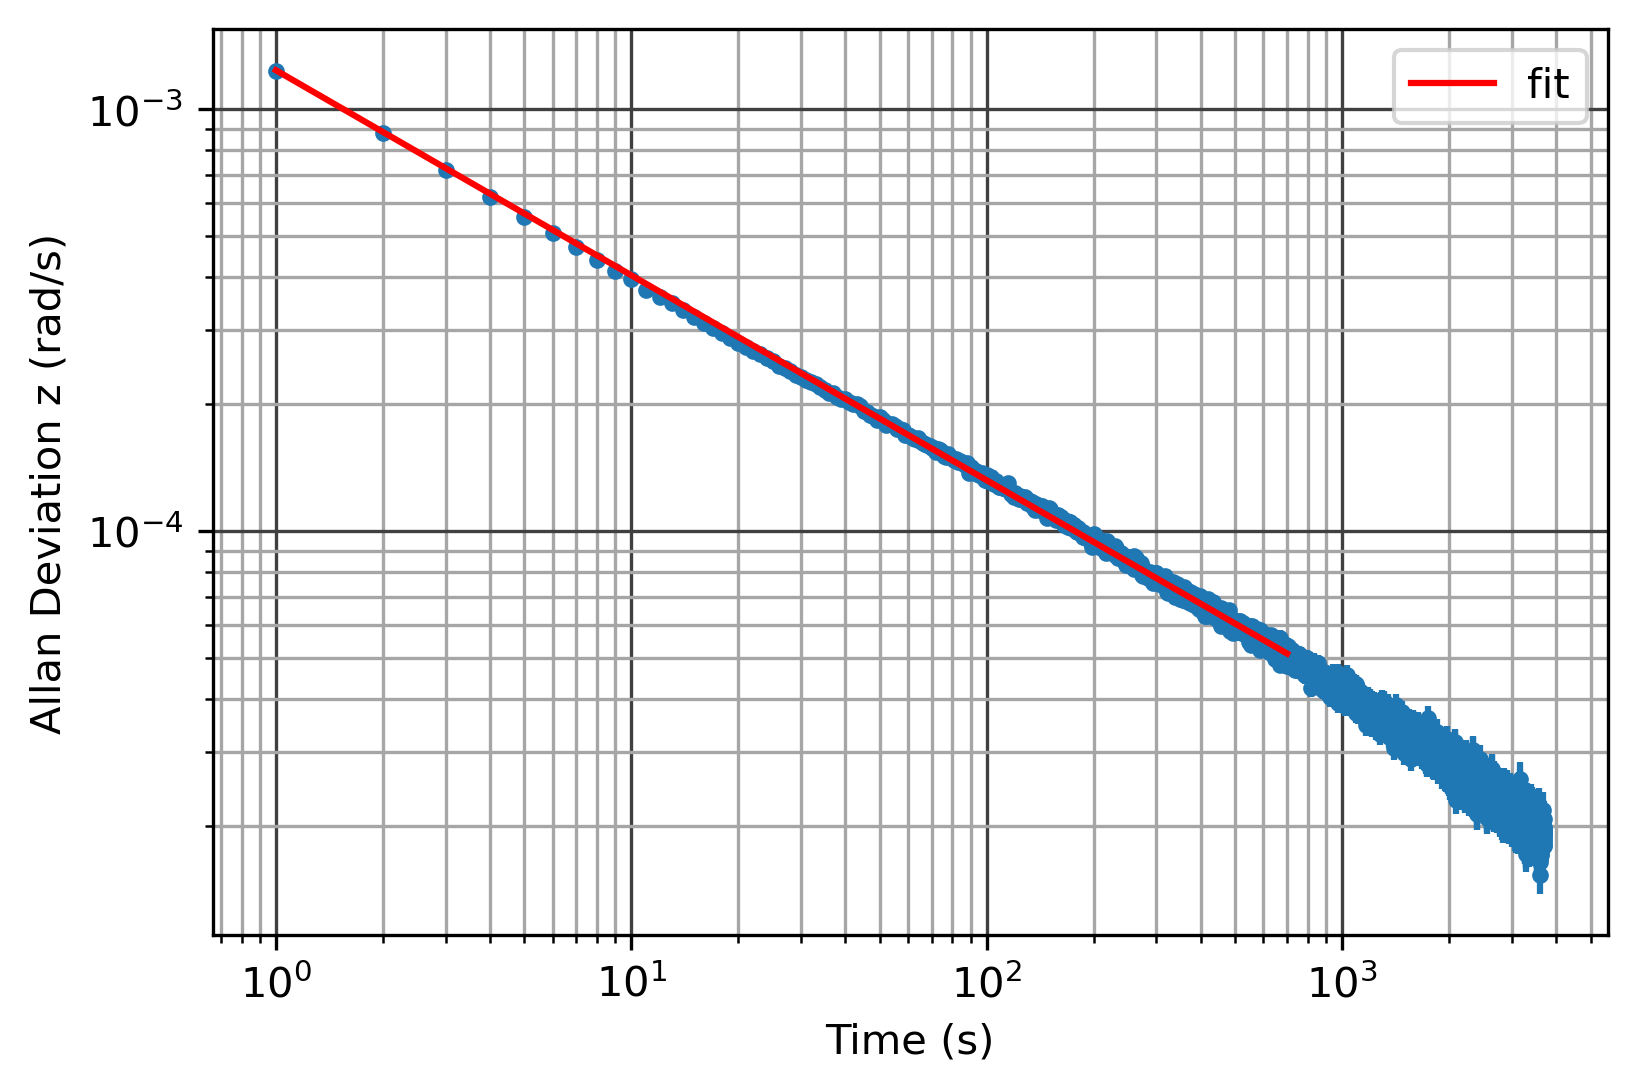
\includegraphics[width=0.4\columnwidth]{allan_z.png}}}
	 \caption{Allan deviation of 3 axes of rotation.}
	 \label{fig:fft}
\end{figure}

We notice that around 700s, the drift becomes larger than the stability, and such indicates the shot-noise time interval. We also do a fit with a slope of -0.5 in order to see this better. Since the Allan deviation is used to quantify the stability of the system over a period of time, we use the value of 700s for doing the measurements for the next part of the homework. 
To calculate the shot noise limited sensitivity, $\mathcal{A}$, we use the formula: 

\begin{equation} \label{eqn:all}
		\sigma_{ad}(\tau) = \frac{\mathcal{A}}{\sqrt{\tau}}
\end{equation}

Using the fact that we plot the Allan deviation with log scale, we solve the Eqn. \ref{eqn:all} to find out that the exponential of the y-intercept should give us the value of $\mathcal{A}$. Because we do not have any readings at the y-intercept, we take the average of the errors for all values of $\tau$ and calculate the error. The results are summarized in the table \ref{tab:A}.

\begin{table}
		\centering
\begin{tabular} {|c|c|}
 \hline
 $A_{x}$ & $0.001389 \pm 0.000004047$ \\
 \hline
 $A_{y}$  & $0.001394 \pm 0.000004203 $ \\
 \hline
 $A_{z}$ & $0.001238 \pm 0.000003919$ \\
 \hline
\end{tabular}
\caption{Shot noise limited sensitivity for different components}
\label{tab:A}
\end{table}

\section{Earth Rotation Rate}

To determine the rotation rate of the Earth, we utilize the same method as we have performed to measure the Allan deviation, but we 
perform this for the shot-time limited interval derived by the section above. \par 

We first measure the gyroscope $x, y, z$ coordinates for the duration of the shot-time interval of $\tau = 700$s. After the data was recorded,
we performed the same measurement but with the phone flipped upside down. This corresponds to a flip in the $y$ direction. 
We then performed the same process but flipping in the $z$-direction instead (i.e. rotations parallel to the surface). This was performed for a 
shorter duration of $\tau = 300$s due to time constraints. The corresponding time series for both results are shown in Fig. \ref{fig:raw_earth_y_faceup}, \ref{fig:raw_earth_y_facedown}, \ref{fig:raw_earth_z_faceup} and \ref{fig:raw_earth_z_facedown}.


\begin{figure}[hbt!]
     \centering
	 {{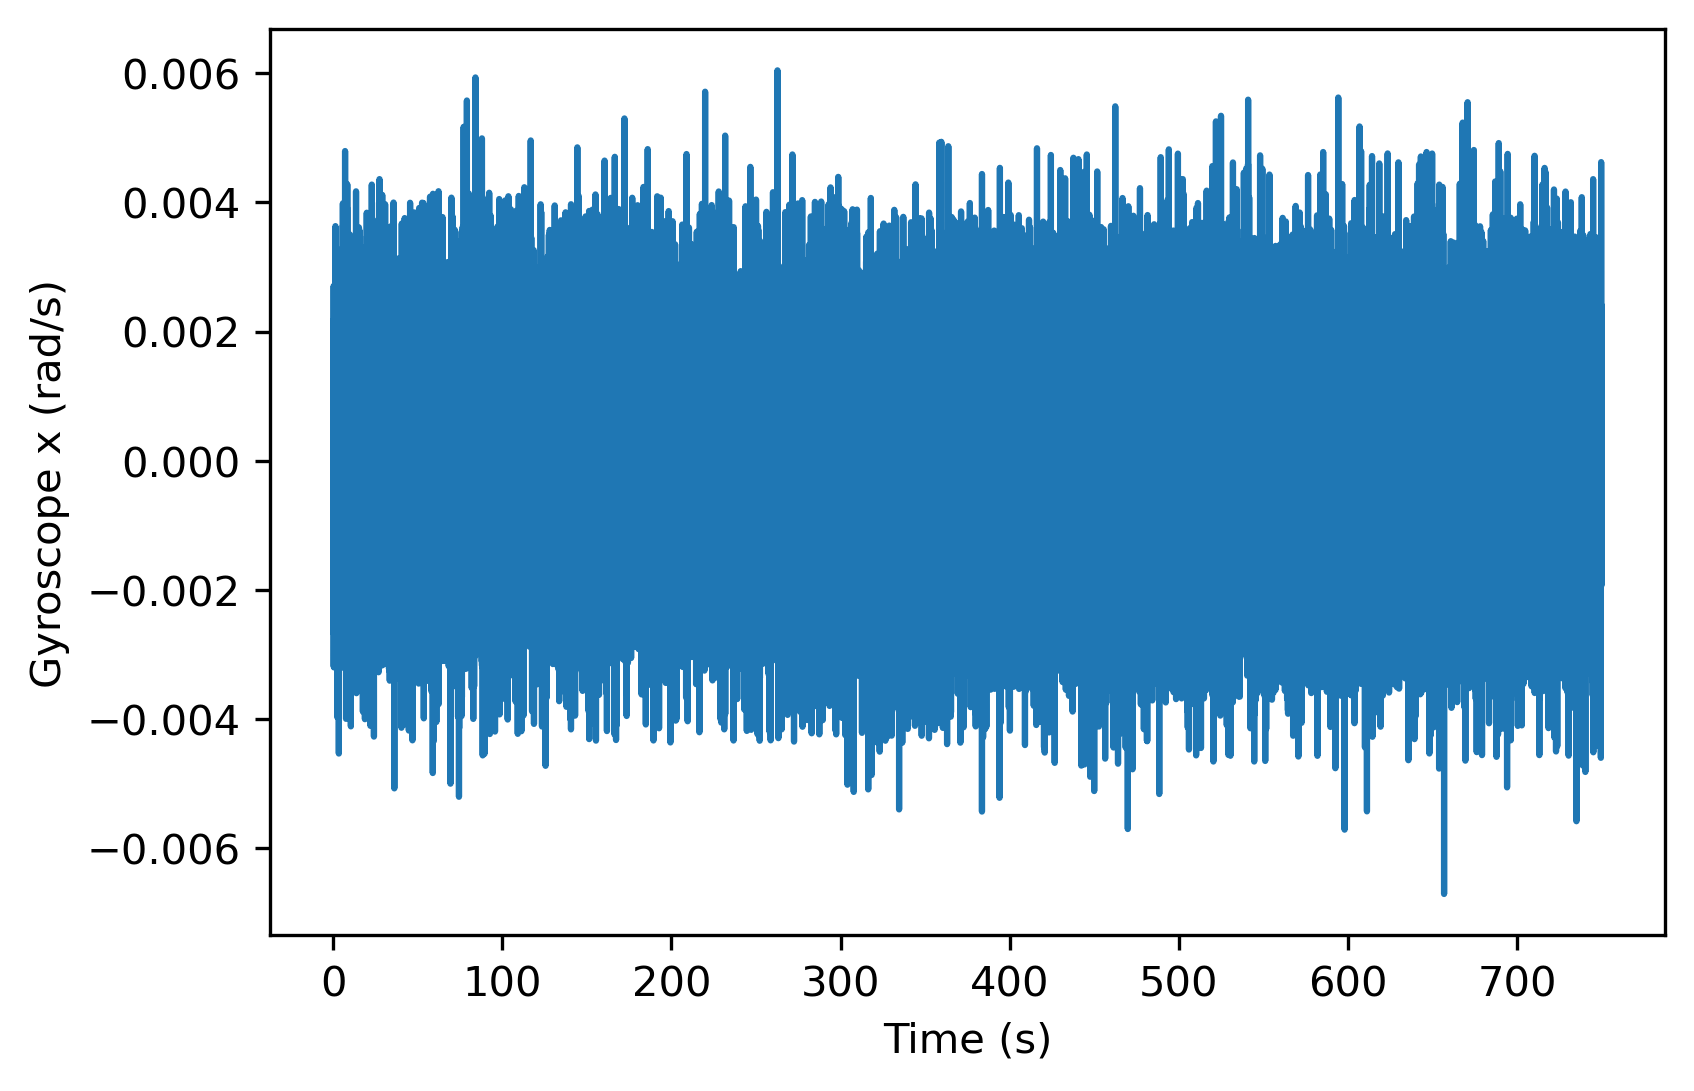
\includegraphics[width=0.4\columnwidth]{raw_ftx.png}}}
	 {{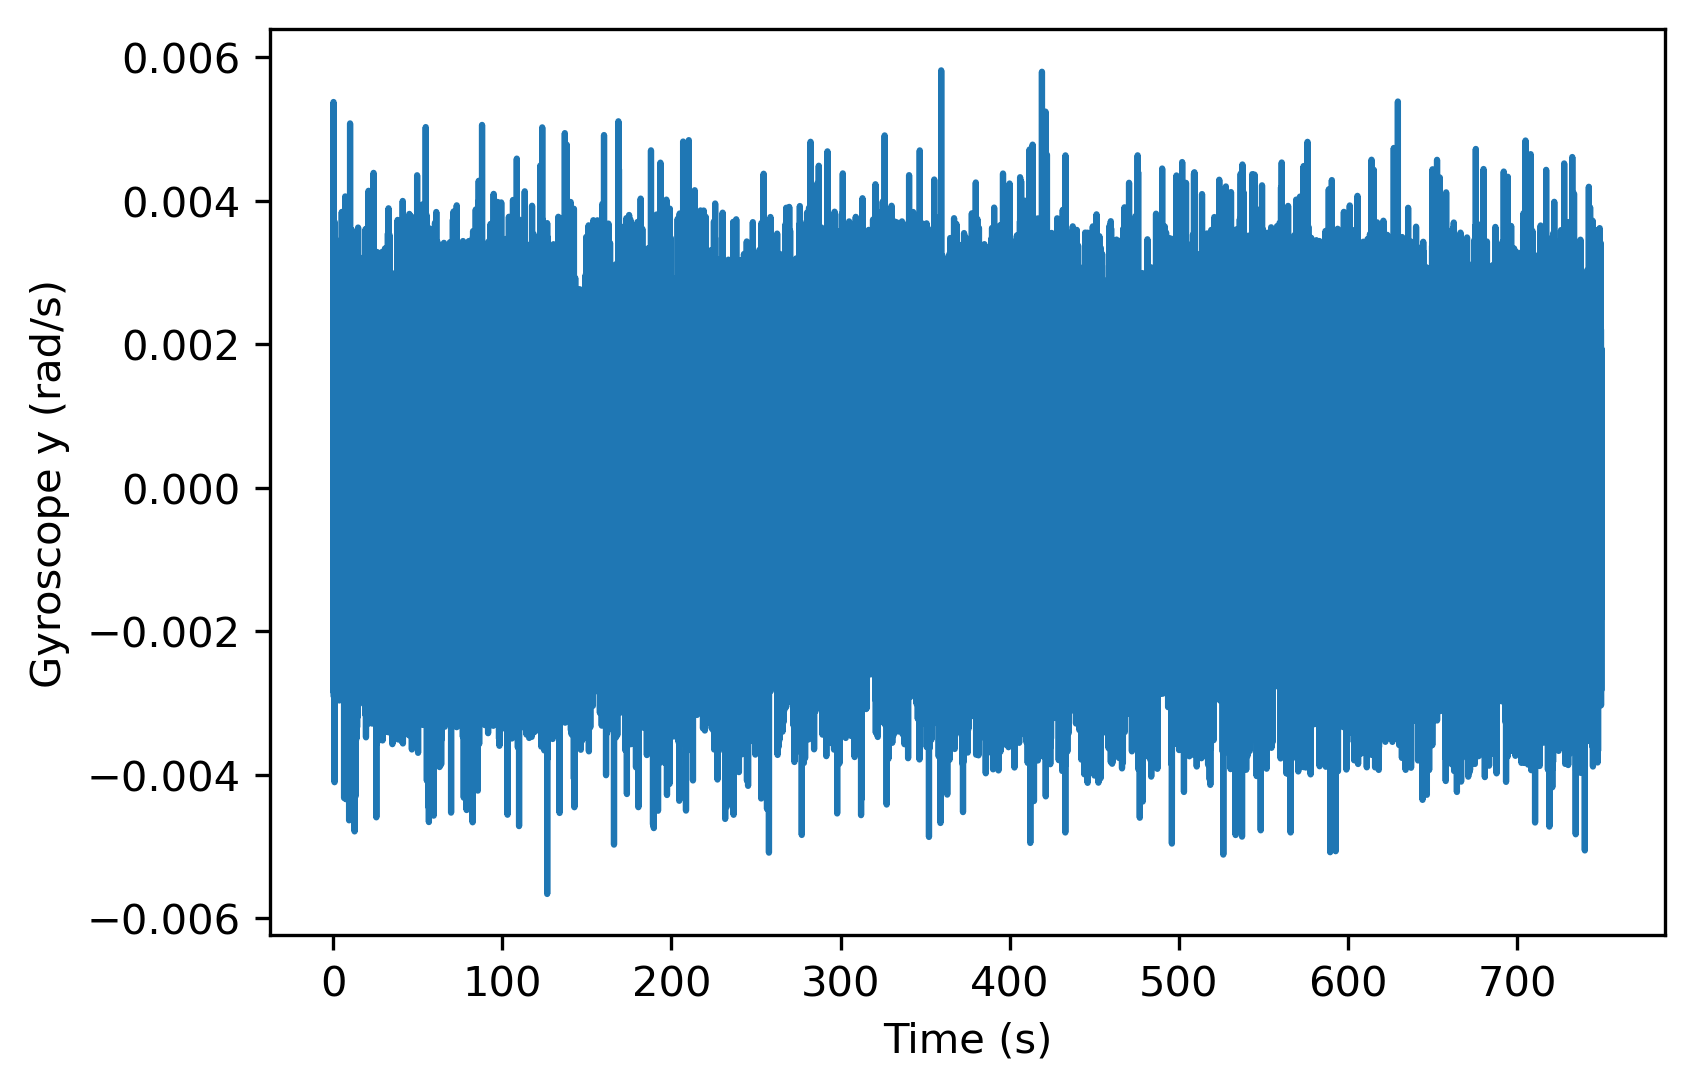
\includegraphics[width=0.4\columnwidth]{raw_fty.png}}}
	 {{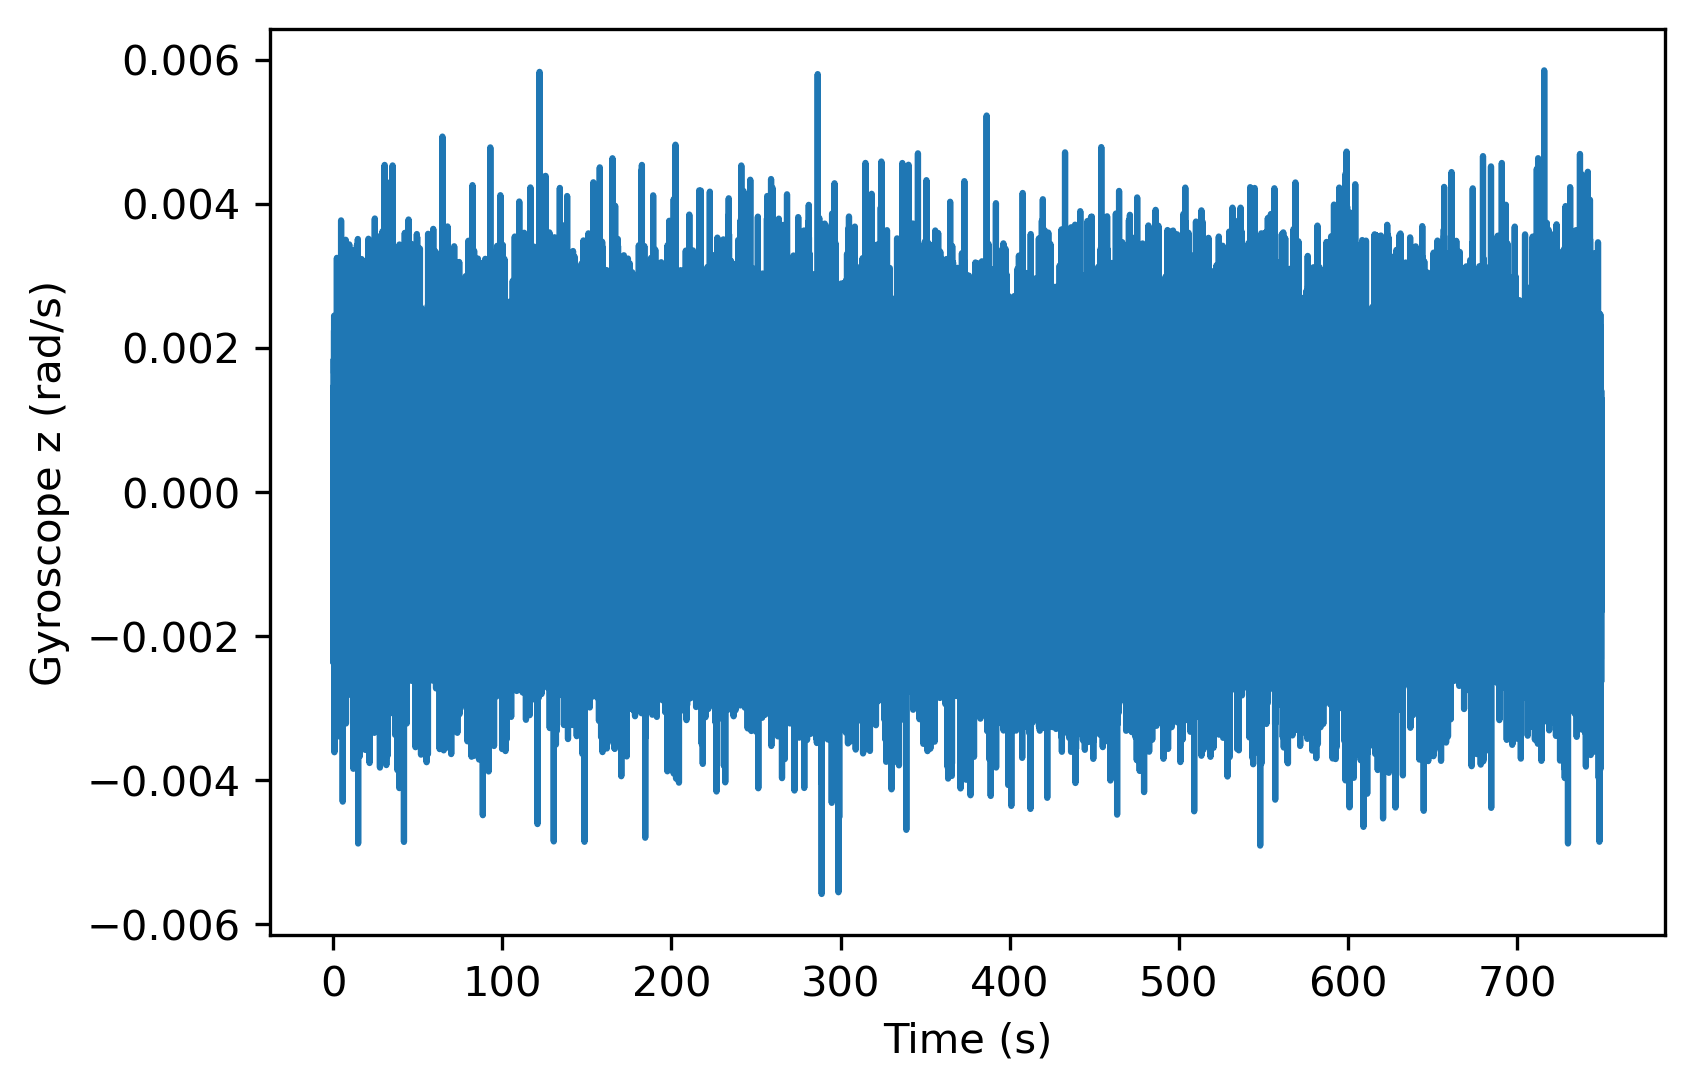
\includegraphics[width=0.4\columnwidth]{raw_ftz.png}}}

     \caption{Raw data of all the three axes of gyroscope from phone for measurement of the Earth's rotation.
               The measurement was took with the phone face up. }
	 \label{fig:raw_earth_y_faceup}
\end{figure}

\begin{figure}[hbt!]
     \centering
     {{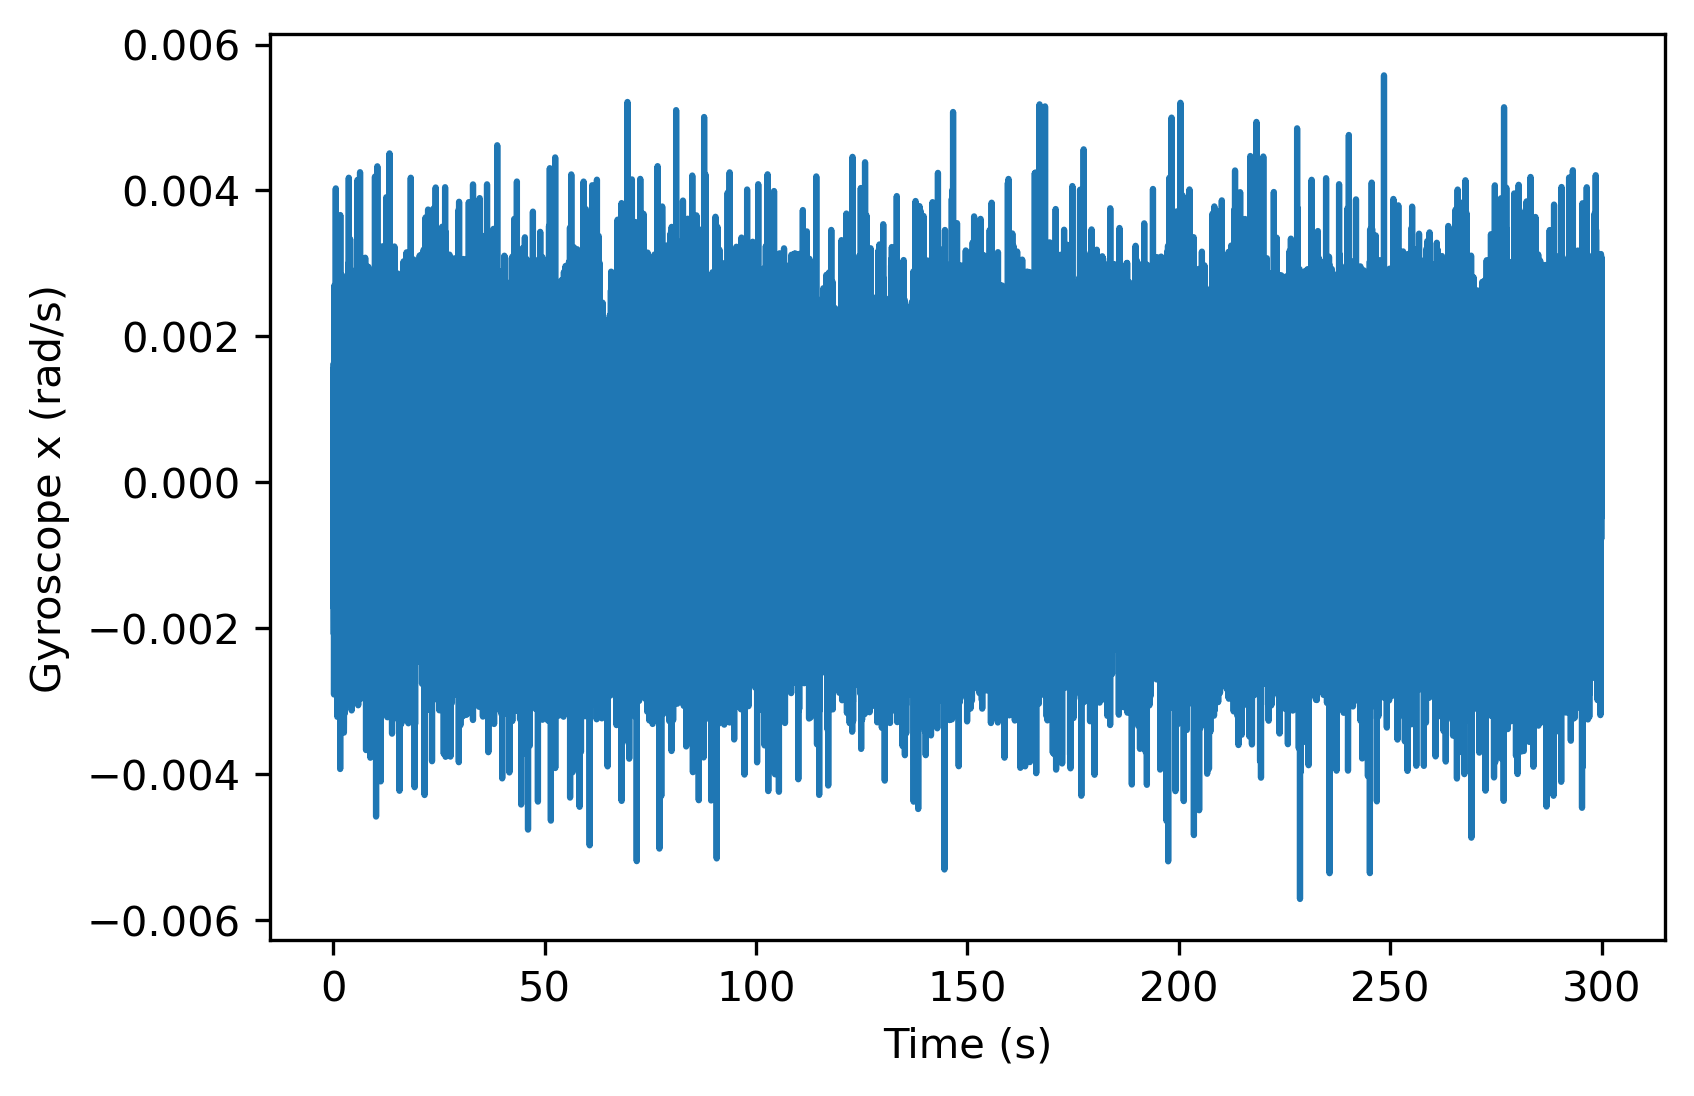
\includegraphics[width=0.4\columnwidth]{raw_btx.png}}}
     {{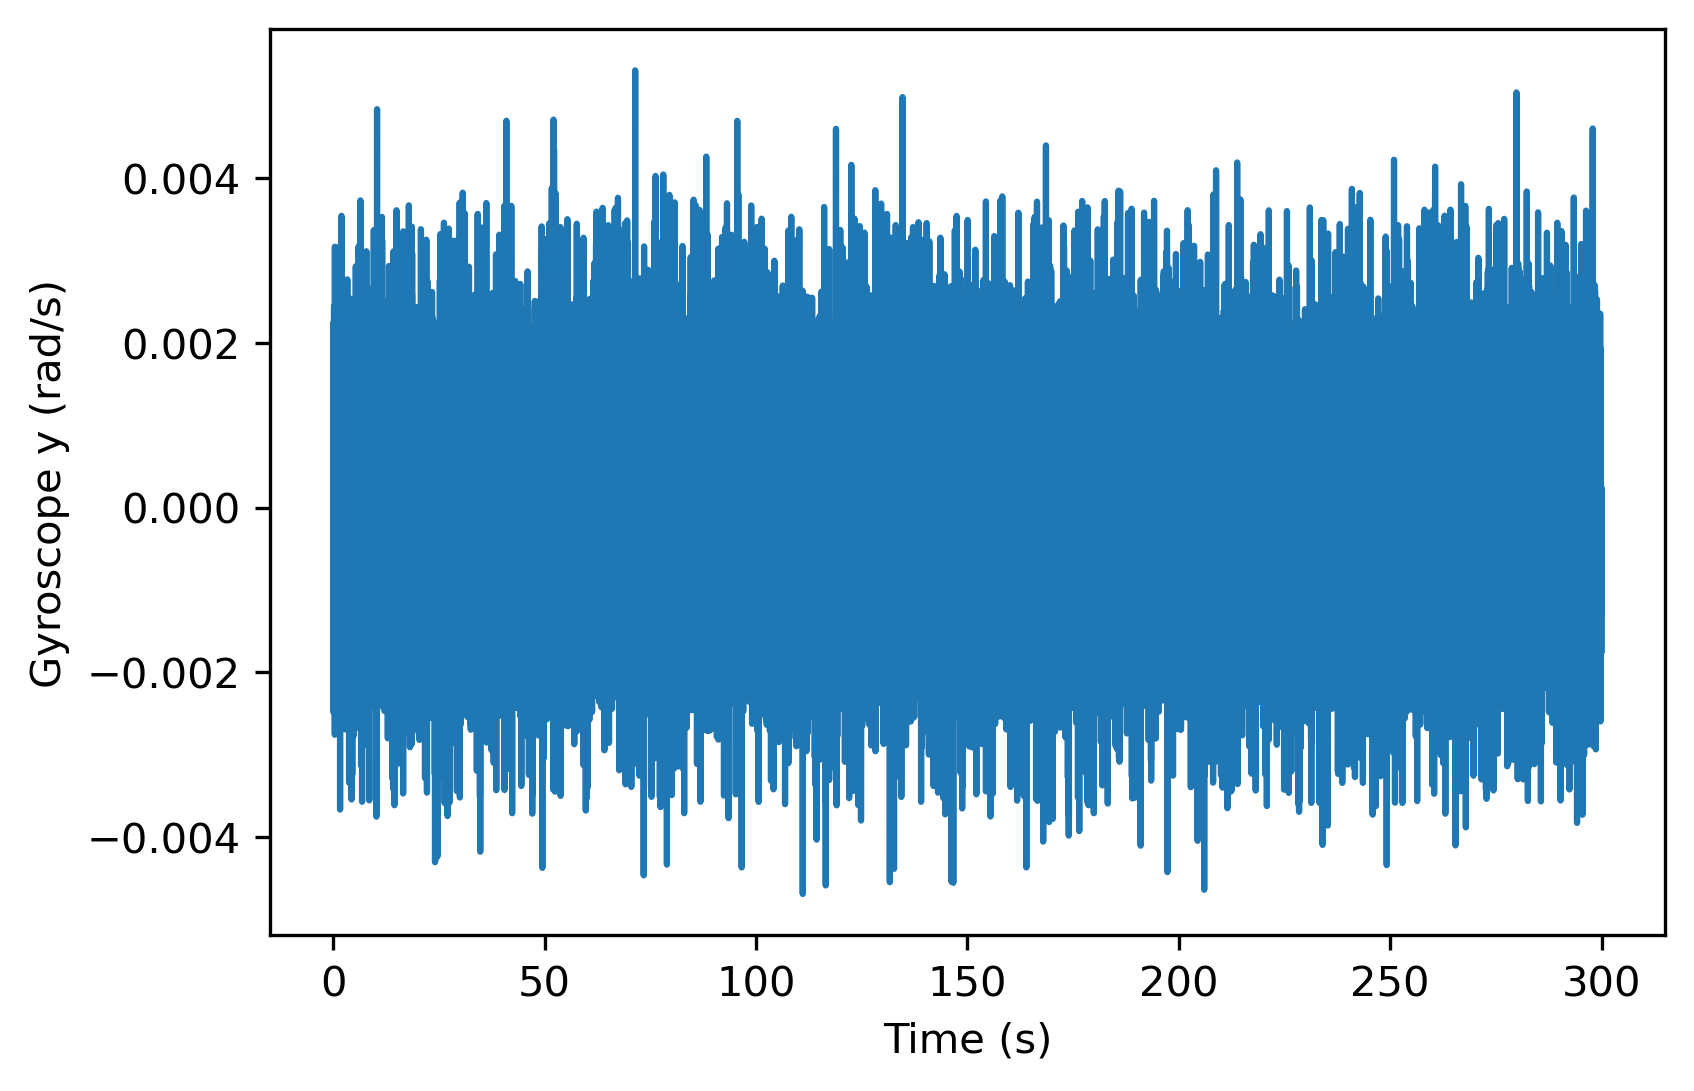
\includegraphics[width=0.4\columnwidth]{raw_bty.png}}}
     {{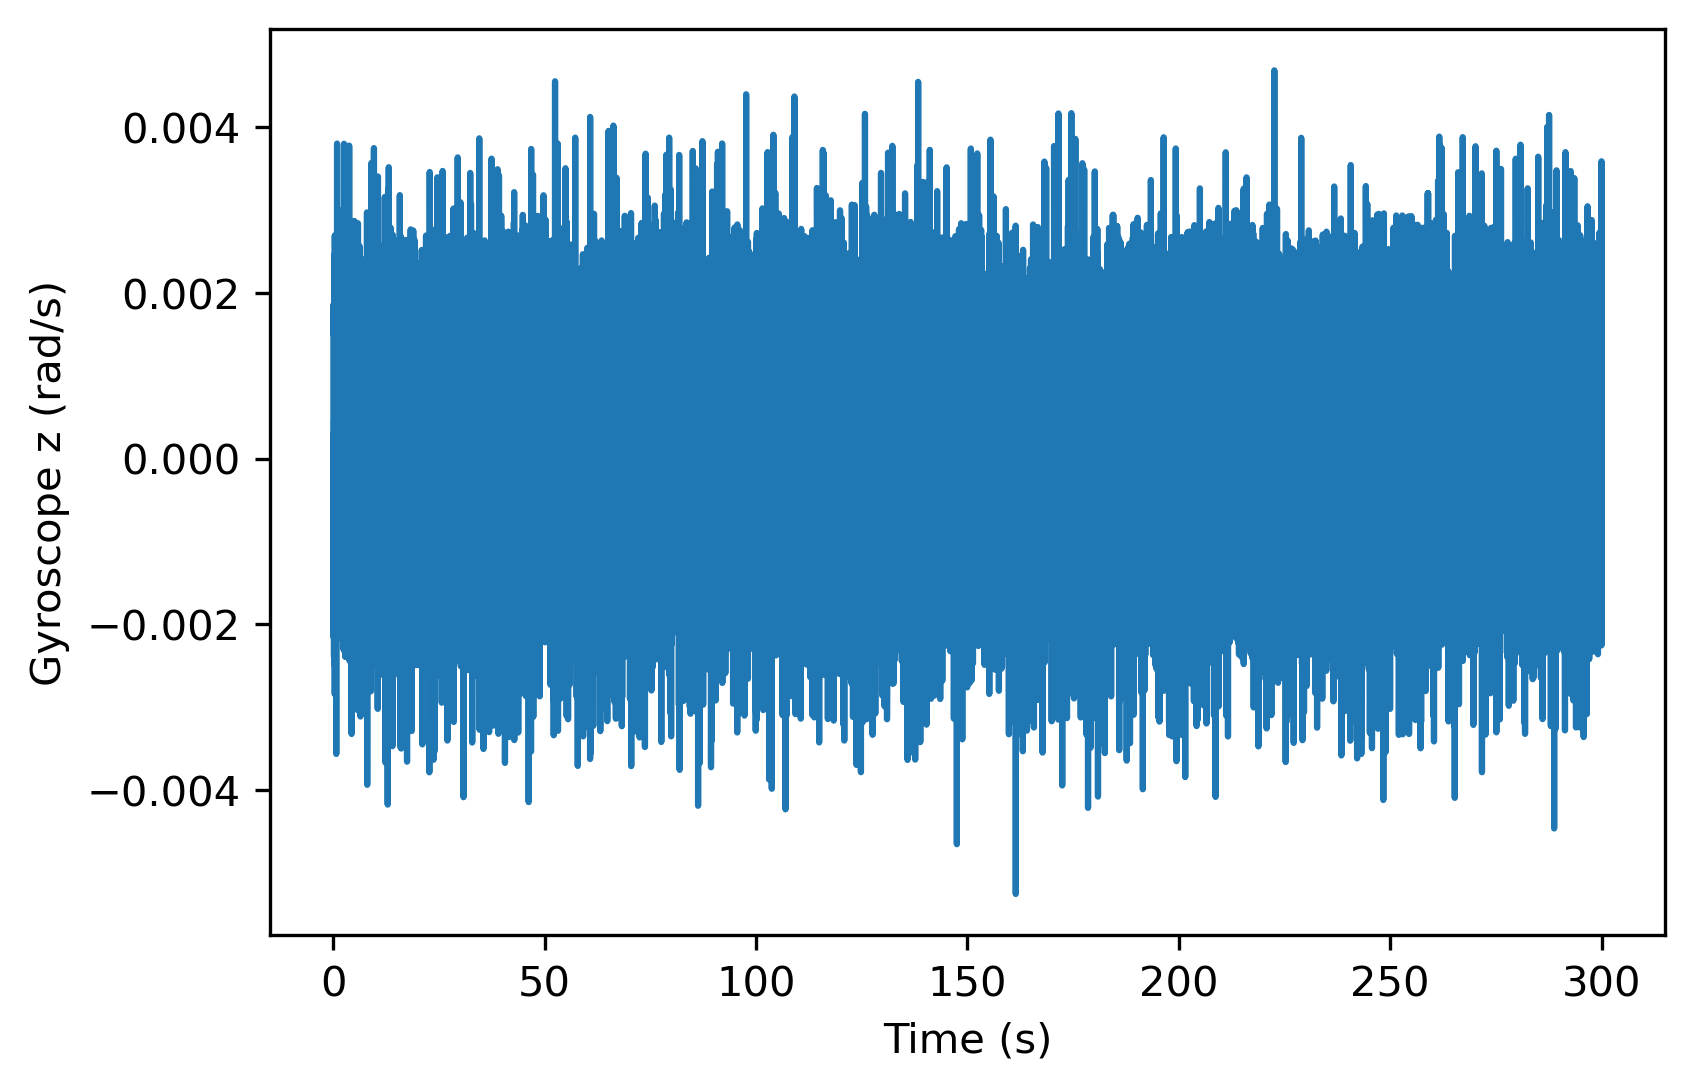
\includegraphics[width=0.4\columnwidth]{raw_btz.png}}}
     \caption{Same as Fig. \ref{fig:raw_earth_y_faceup} but for phone face down instead.}
     \label{fig:raw_earth_y_facedown}
\end{figure}

\begin{figure}[hbt!]
     \centering
	 {{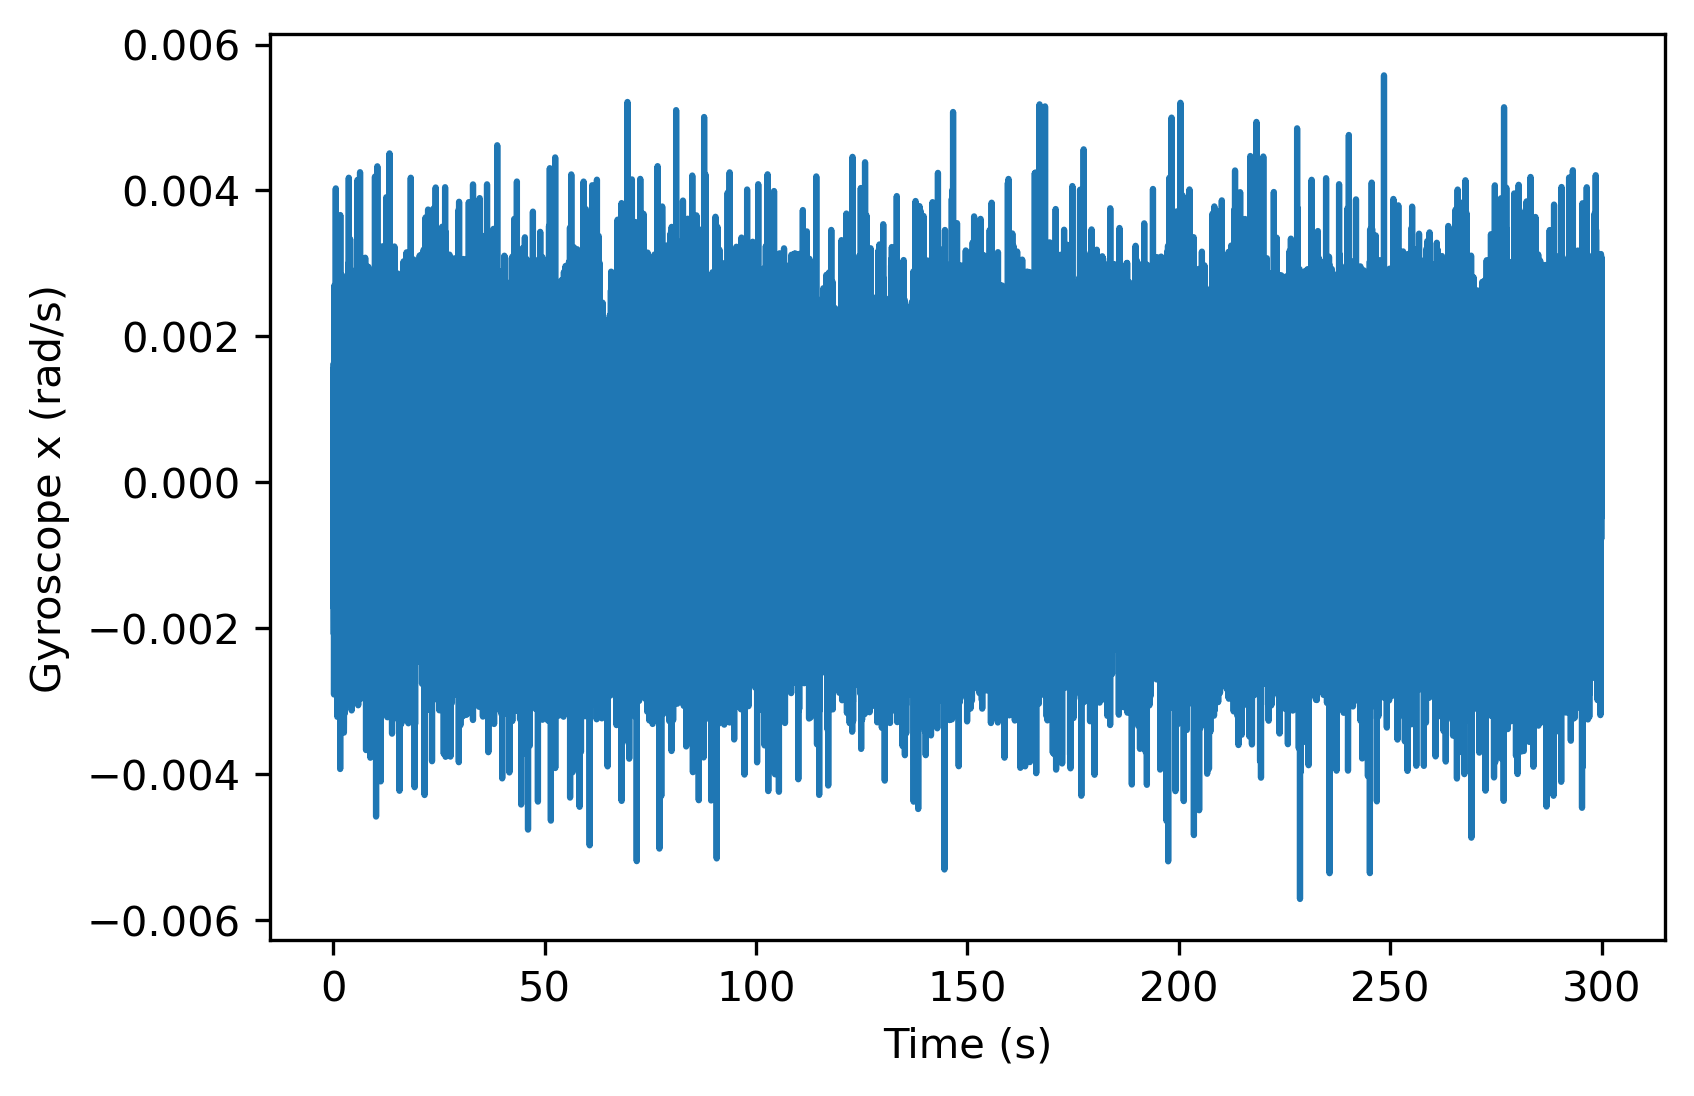
\includegraphics[width=0.4\columnwidth]{raw_okx.png}}}
	 {{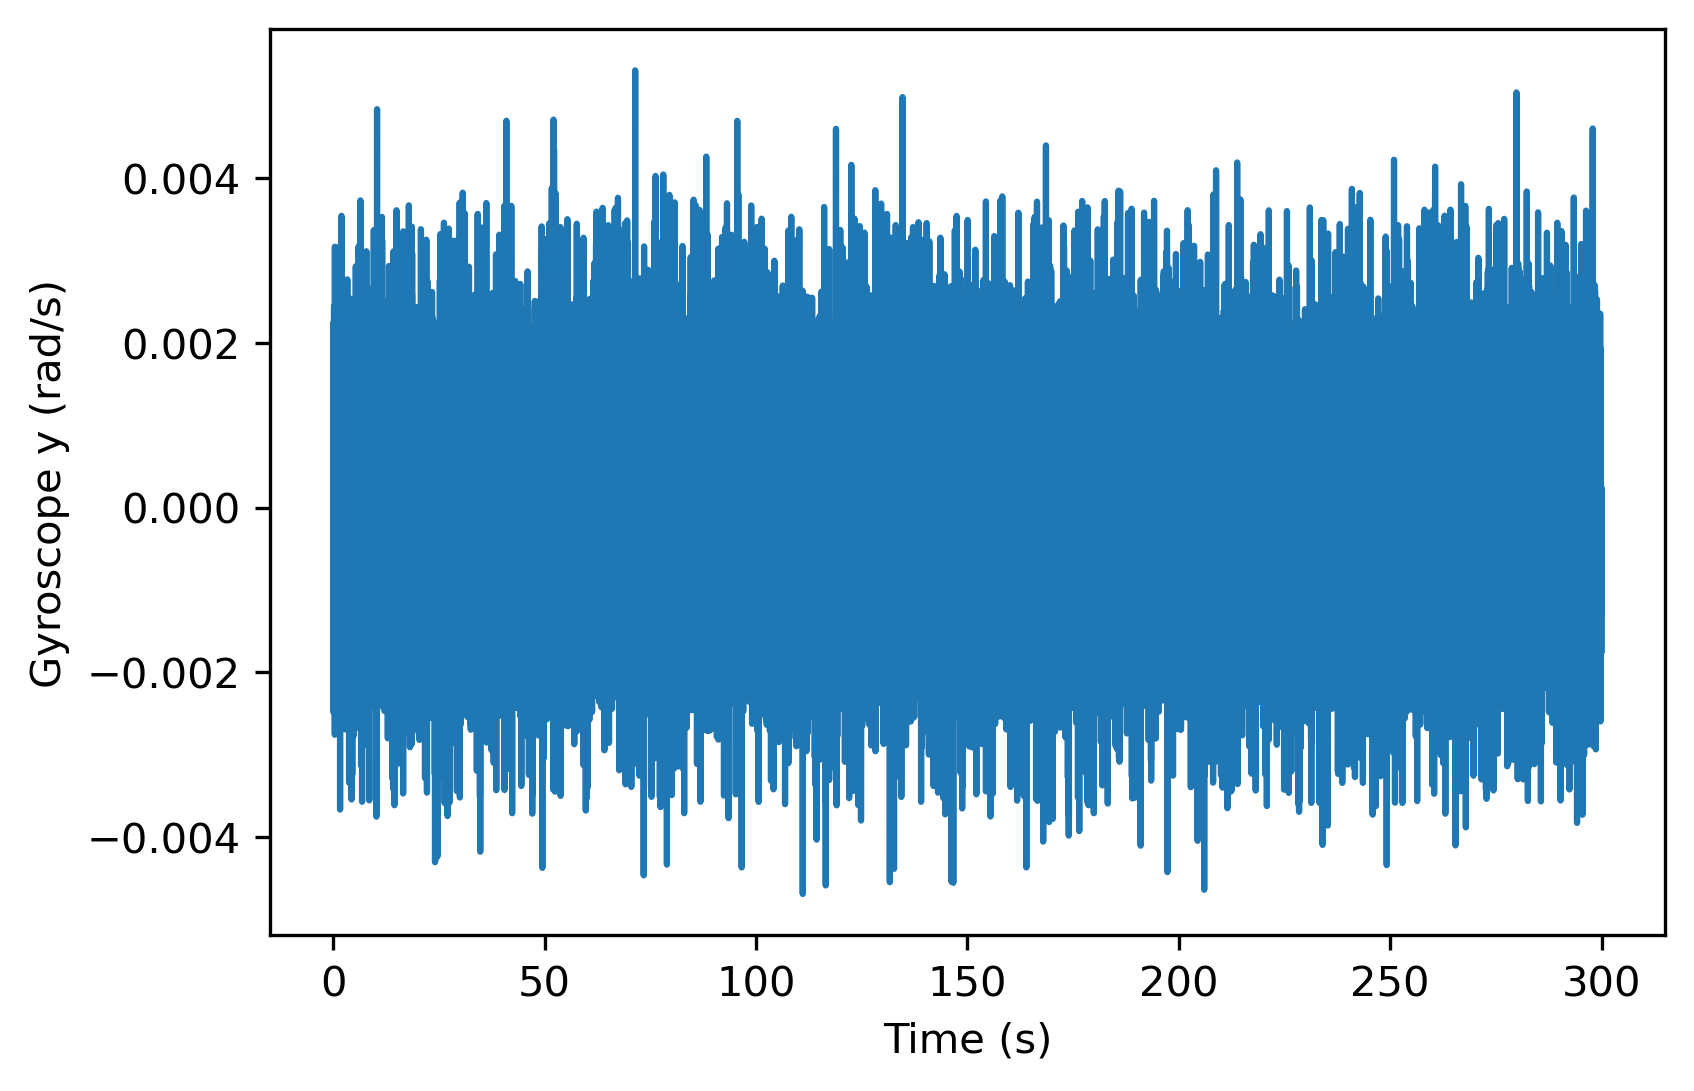
\includegraphics[width=0.4\columnwidth]{raw_oky.png}}}
	 {{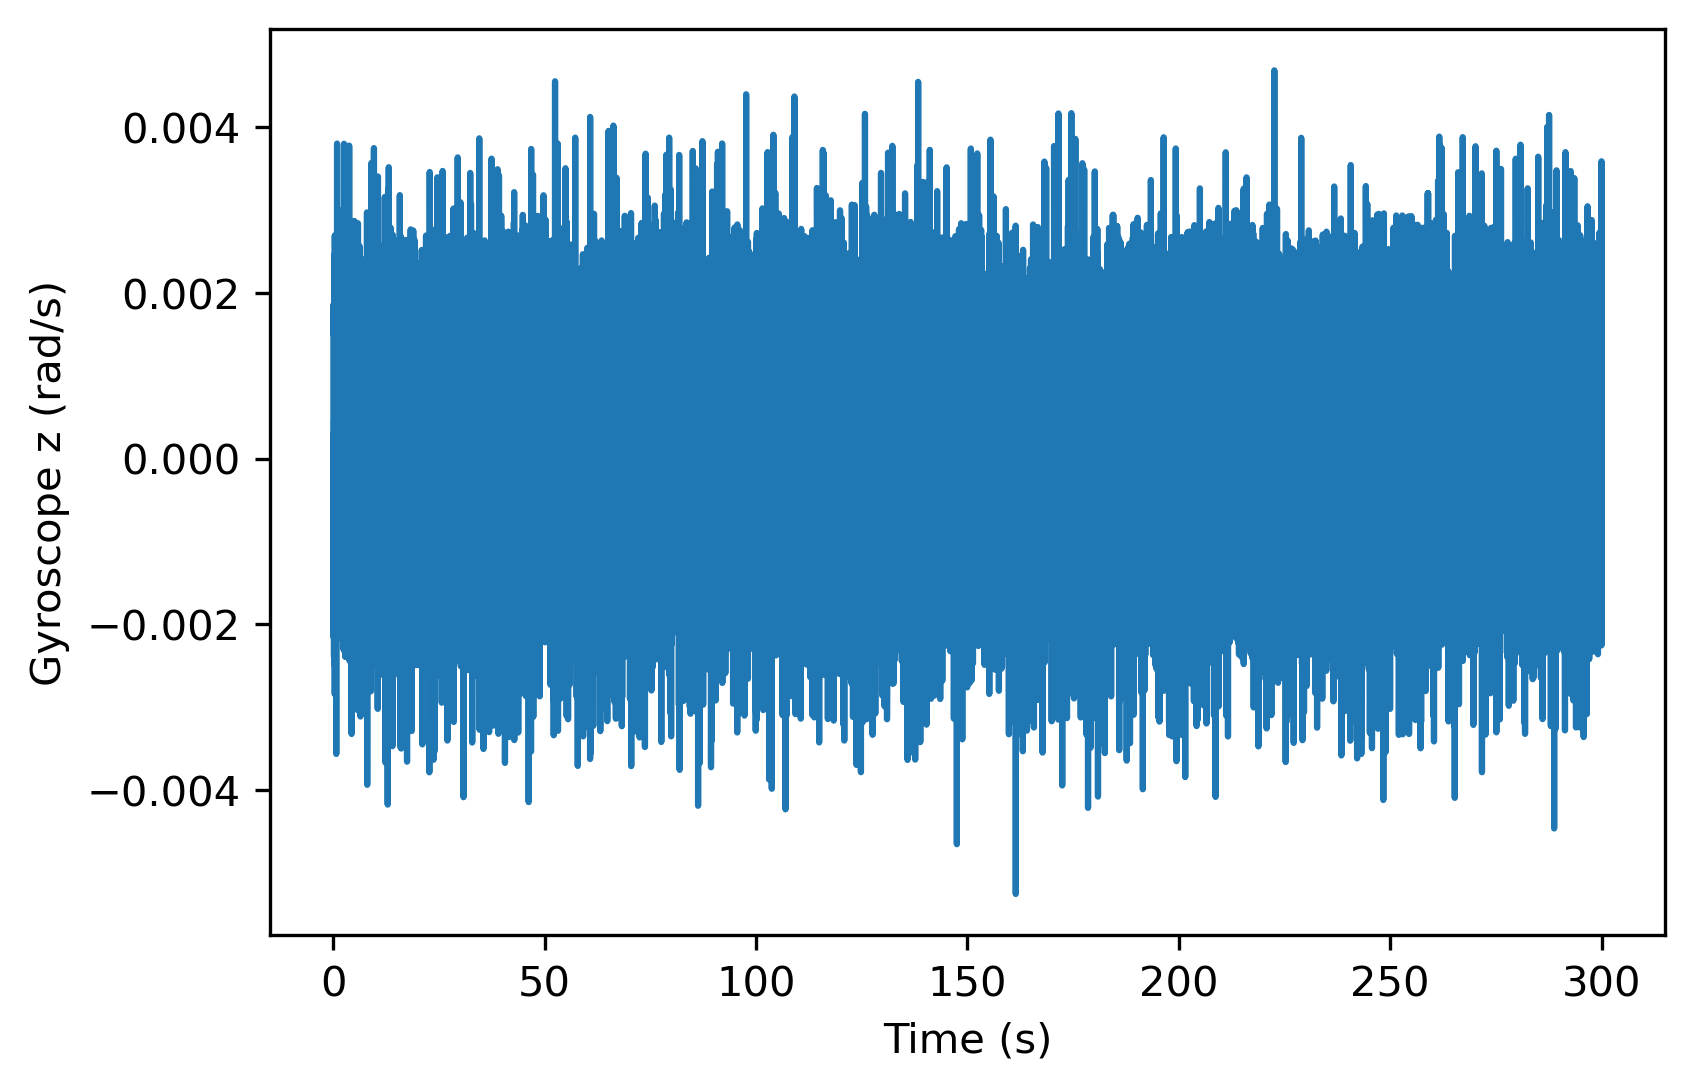
\includegraphics[width=0.4\columnwidth]{raw_okz.png}}}

     \caption{Same as Fig. \ref{fig:raw_earth_y_faceup} but for rotations in the $z$-direction. This was performed 
               with the phone facing towards the South Pole. }
	 \label{fig:raw_earth_z_faceup}
\end{figure}

\begin{figure}[hbt!]
     \centering
     {{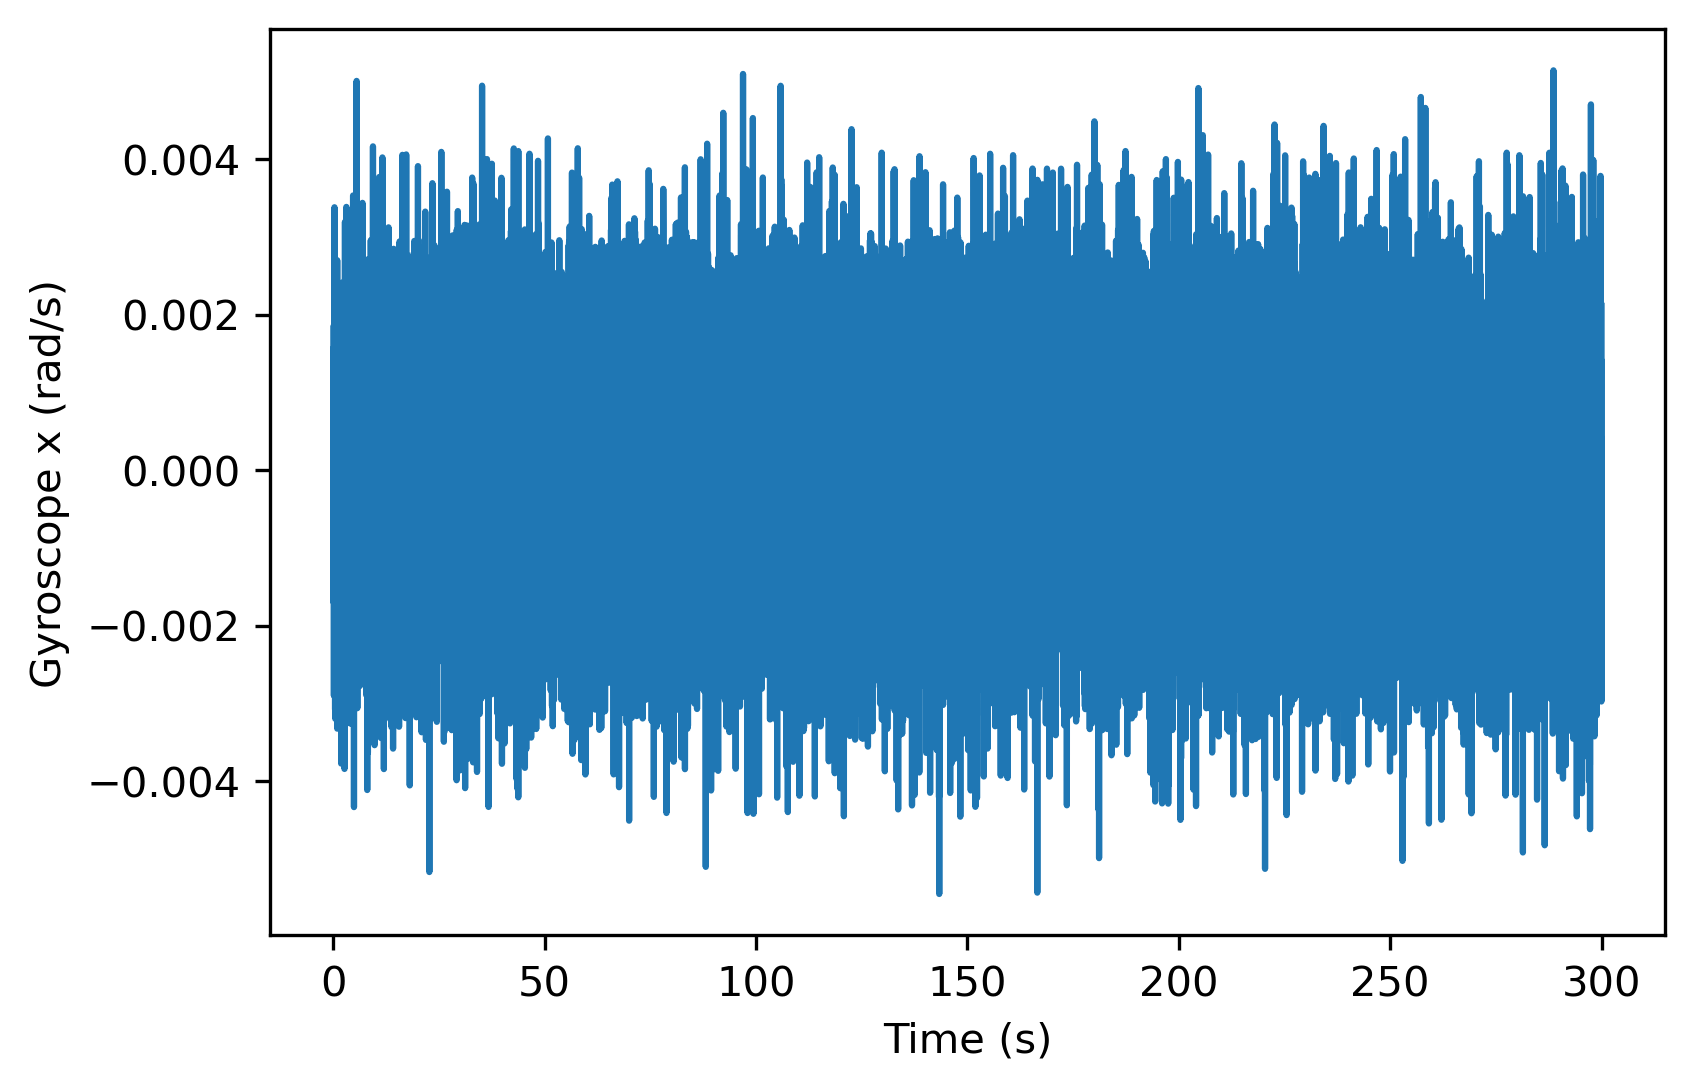
\includegraphics[width=0.4\columnwidth]{raw_180kx.png}}}
     {{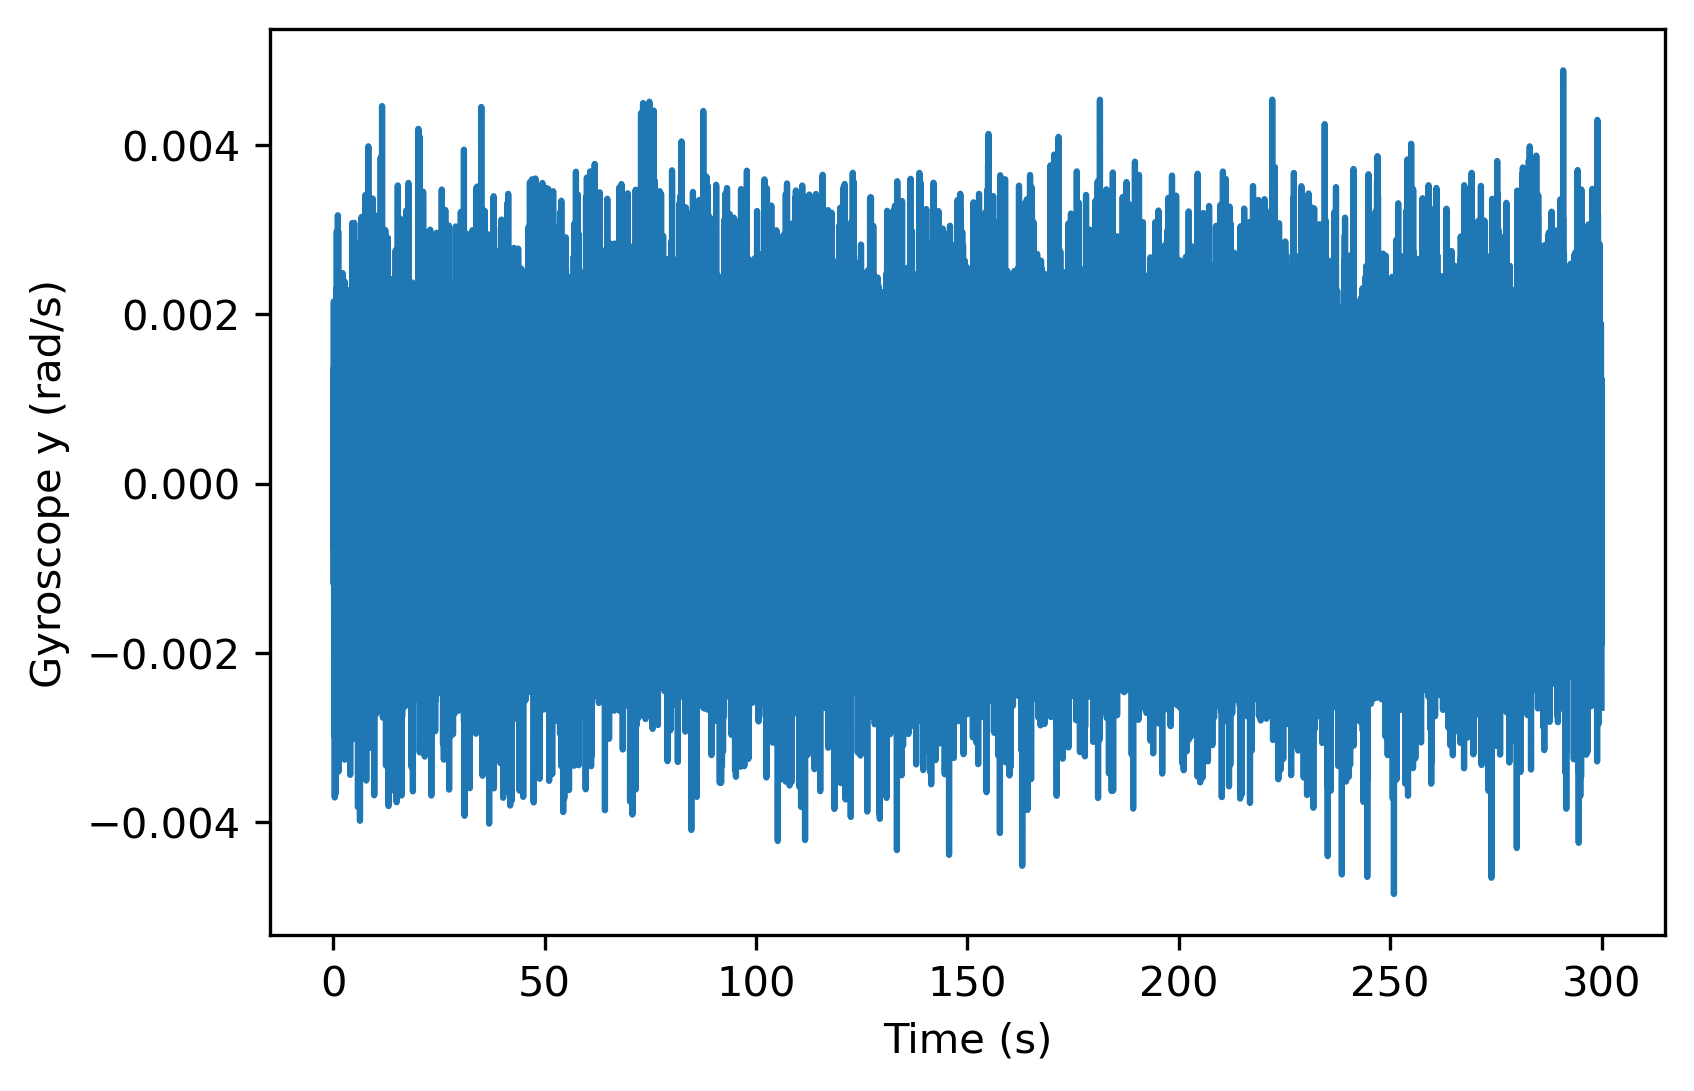
\includegraphics[width=0.4\columnwidth]{raw_180ky.png}}}
     {{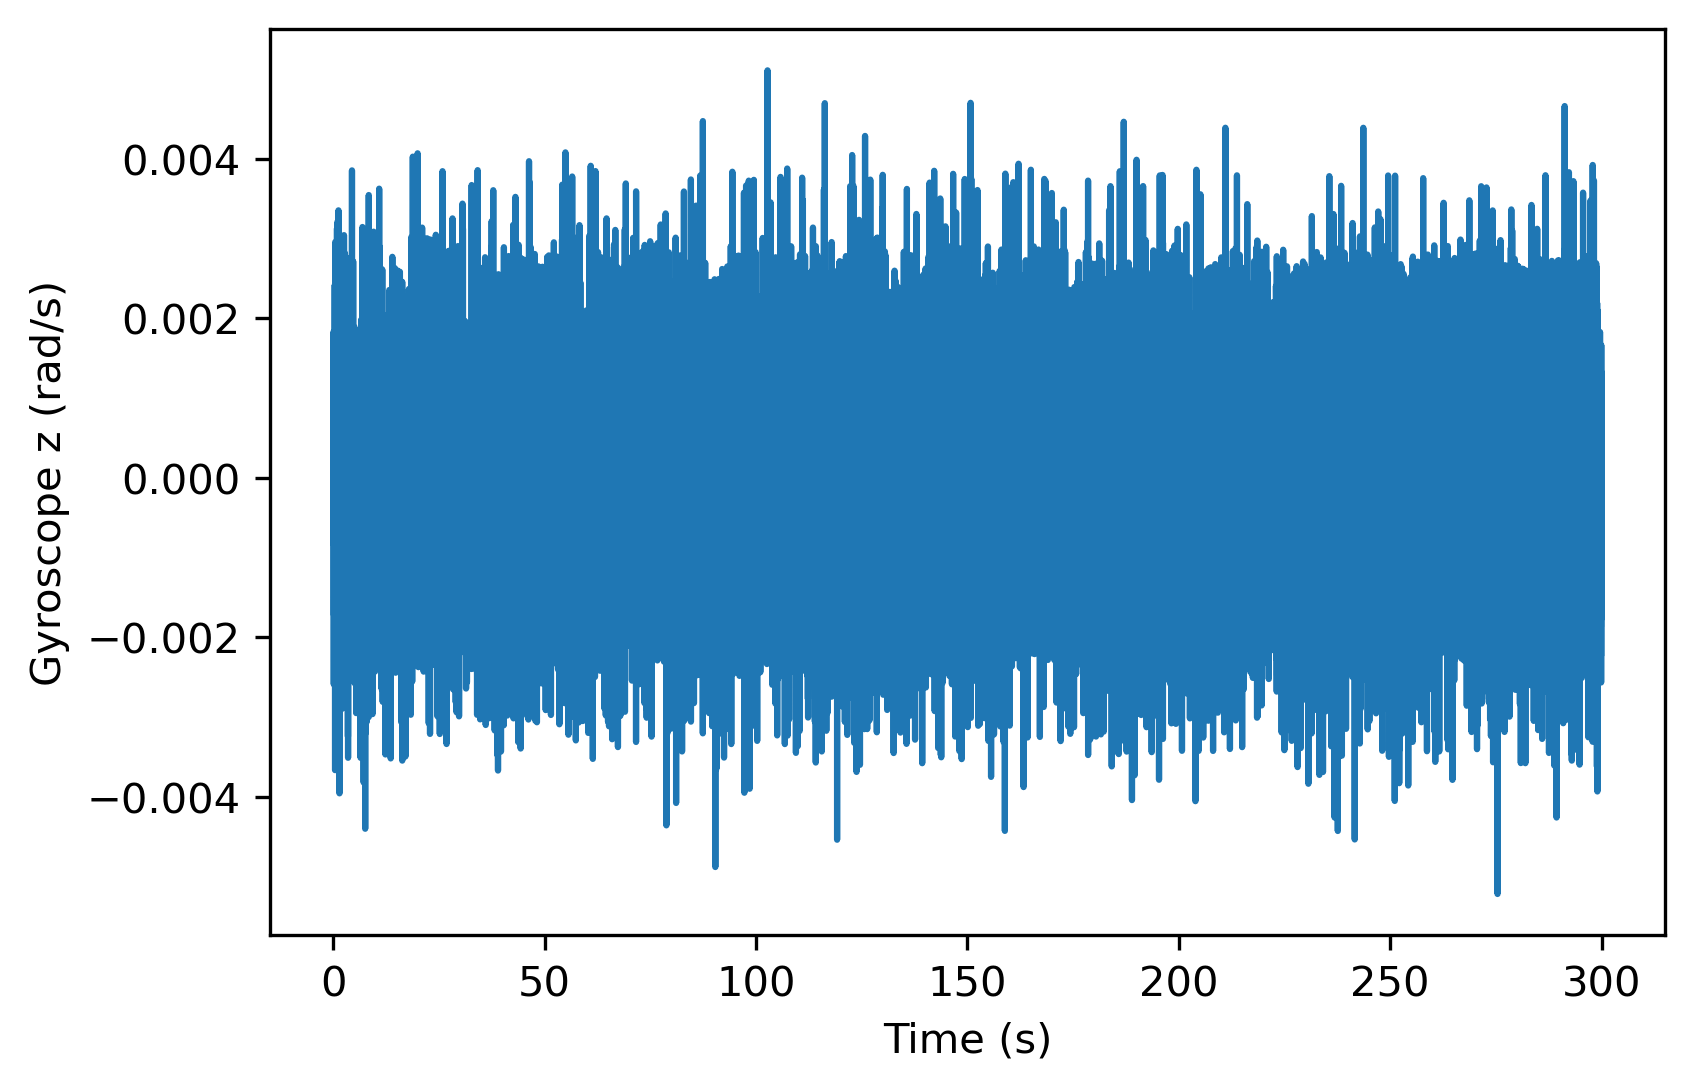
\includegraphics[width=0.4\columnwidth]{raw_180kz.png}}}
     \caption{Same as Fig. \ref{fig:raw_earth_z_faceup} but for those facing towards the North Pole instead.}
     \label{fig:raw_earth_z_facedown}
\end{figure}


After performing the FFT onto the resulting time series, we observed the sharp peak in the gyroscope $x$-direction.
This shows that there is a clear bias in the $x$-direction of the phone gyroscope. 

The temporal average of each measurement (both flipped and unflipped) was taken, and the difference between the unflipped and flipped
measurements were taken (normalized by 2). For example, for the $x$ coordinate we have: 
\begin{equation}
     \delta \bar{\omega_x} = \frac{|\bar{x}_{noflip} - \bar{x}_{flip}|}{2}
\end{equation}

Such measurements for both rotations are tabulated on Table \ref{tab:avg_rate_xyz}. The magnitude of the values are also evaluated.
Note that for arbitrarily small differences, the deviations may be small and thus to properly normalize this, one needs to take
into arround the uncertainty in the measurement as well. 

\begin{table}
\centering
\begin{tabular} {|c|c|c|}
 \hline
 Coordinate & $\delta \bar{\omega_i}$, face up/down (rad/s) & $\delta \bar{\omega_i}$, face North/South (rad/s) \\
 \hline
 $x$ & $\num{9.273e-8}$ & $\num{9.956e-6}$ \\
 \hline
 $y$  & $\num{4.603e-7}$ & $\num{2.814e-5}$ \\
 \hline
 $z$ & $\num{2.340e-6}$ & $\num{3.357e-6}$  \\
 \hline
 $\omega$ & $\num{2.386e-6}$ & $\num{3.004e-5}$ \\
 \hline
\end{tabular}
\caption{Difference of temporal average of rotation rate for each gyroscopic coordinate and its magnitude. }
\label{tab:avg_rate_xyz}
\end{table}
 
Furthermore, to properly account for the Earth's rotation rate, we need to transform from the local frame in which we observe the phone's orientation in.
This can be done by a simple coordinate transformation as such: $\omega = \Omega_E \cos\phi$, where $\phi$ is the geographic latitude.
With $\phi = \SI{39.257}{\degree}$ (defined from the North Pole), we obtain our corrected rotation rate of the Earth as 
$\Omega_E = 3.083\mu \text{rad}s^{-1}$ and $\Omega_E = 38.80\mu \text{rad}s^{-1}$ for the up/down and North/South
flip case respectively.  \par 

When comparing the values of the rotation rate to the analytical value $\Omega_{E, thr} = 72.92\mu \text{rad}s^{-1}$, 
both yielded values are underestimated. However, the rate where the phone was flipped upside down yielded lower values
compared to that when we flipped the phone from South to North. This indicates a clear bias in the rotation and how it 
impacts the measurement, which is clear due to the East-West rotation of the Earth. \par 

Furthermore, the underestimation of the values are clear due to the various systematical uncertainties that need to be accounted for.
The movement of nearby people, the wind, the temperature differences can all impact the phone gyroscope in some way. The 
MEMS gyroscope does not have as many tools that will calibrate for such deviations as compared to our experimental setup. 
% We also evaluated the magnitude of such values to determine the magnitude of the rotation rate, yielding $\omega = \SI{2.386e-6}{\rad\per\second}$.




\begin{comment}
\newpage
\section{Appendix}

Below the raw data imported from the \texttt{phyphox} application for fast rotations in the $+y$ direction (corresponding to the time series in \ref{fig:gyro_plot_fast_y}) 
is shown.

% \begin{table}[!ht]
%     \centering
\setlength\LTleft{0pt}
\setlength\LTright{0pt}

\begin{longtable}{|c|c|c|c|c|}
\hline
Time (s) & Gyroscope x \newline (rad/s) & Gyroscope y \newline (rad/s) & Gyroscope z \newline (rad/s) & Absolute \newline (rad/s) \\ \hline
    6.767499995E-3 & -1.010426786E-2 & -2.324782610E-1 & -8.401471376E-2 & 2.473998993E-1 \\ \hline
    1.681750000E-2 & -4.476520233E-3 & -2.514493167E-1 & -1.048773974E-1 & 2.724813142E-1 \\ \hline
    2.686650000E-2 & -5.002761260E-3 & -2.558797300E-1 & -1.042318493E-1 & 2.763399035E-1 \\ \hline
    3.691650000E-2 & -1.232061721E-2 & -2.315417826E-1 & -1.004440412E-1 & 2.526903245E-1 \\ \hline
    4.696550000E-2 & -1.514143683E-2 & -2.187458277E-1 & -9.285589308E-2 & 2.381201737E-1 \\ \hline
    5.701449999E-2 & -3.160101548E-2 & -2.359628826E-1 & -9.338636696E-2 & 2.557305607E-1 \\ \hline
    6.706450000E-2 & -4.849477857E-2 & -2.816651165E-1 & -1.120228991E-1 & 3.069790080E-1 \\ \hline
    7.711350000E-2 & -4.799867794E-2 & -3.520550728E-1 & -1.132196411E-1 & 3.729146477E-1 \\ \hline
    8.716250000E-2 & -4.955183342E-2 & -4.466729164E-1 & -1.066344455E-1 & 4.618906618E-1 \\ \hline
    9.721250000E-2 & -7.474593818E-2 & -4.910189509E-1 & -1.147160977E-1 & 5.097512614E-1 \\ \hline
    1.072615000E-1 & -1.012153625E-1 & -4.642693698E-1 & -1.109495908E-1 & 4.879553351E-1 \\ \hline
    1.173105000E-1 & -1.143684387E-1 & -4.120182097E-1 & -8.564193547E-2 & 4.360890804E-1 \\ \hline
    1.273605000E-1 & -1.186878234E-1 & -3.871080875E-1 & -7.599277049E-2 & 4.119640422E-1 \\ \hline
    1.374095000E-1 & -1.142060608E-1 & -3.996090293E-1 & -7.642972469E-2 & 4.225776892E-1 \\ \hline
    1.474595000E-1 & -1.142915487E-1 & -4.720688462E-1 & -4.730672389E-2 & 4.880056145E-1 \\ \hline
    1.575085000E-1 & -1.201705858E-1 & -5.596361160E-1 & 6.058456376E-3 & 5.724248920E-1 \\ \hline
    1.675575000E-1 & -9.741094708E-2 & -5.834802389E-1 & 6.109268218E-2 & 5.947019402E-1 \\ \hline
    1.776075000E-1 & -8.800595254E-2 & -4.699653685E-1 & 1.133963764E-1 & 4.913972257E-1 \\ \hline
    1.876565000E-1 & -7.030151784E-2 & -2.996791303E-1 & 1.166337207E-1 & 3.291706387E-1 \\ \hline
    1.977055000E-1 & -5.914305523E-2 & -2.122400105E-1 & 7.882495224E-2 & 2.340023422E-1 \\ \hline
    2.077555000E-1 & -3.155750036E-2 & -2.722881734E-1 & 5.201544613E-2 & 2.790023868E-1 \\ \hline
    2.178045000E-1 & 9.016429074E-3 & -4.376586080E-1 & 3.718788177E-2 & 4.393282277E-1 \\ \hline
    2.278545000E-1 & 4.824479297E-2 & -5.677084327E-1 & 3.008522838E-2 & 5.705484603E-1 \\ \hline
    2.379035000E-1 & 7.523760945E-2 & -4.890623689E-1 & 3.054252826E-2 & 4.957575461E-1 \\ \hline
    2.479525000E-1 & 8.370779455E-2 & 2.174204681E-3 & 8.641111851E-2 & 1.203270686E-1 \\ \hline
    2.580025000E-1 & 9.438323975E-2 & 1.216244459E0 & 2.356295884E-1 & 1.242449228E0 \\ \hline
    2.680515000E-1 & -7.097269595E-2 & 3.820101738E0 & 5.026485324E-1 & 3.853682649E0 \\ \hline
    2.781005000E-1 & -5.254991651E-1 & 9.453613281E0 & 5.492578149E-1 & 9.484125558E0 \\ \hline
    2.881505000E-1 & -5.141525269E-1 & 1.864735222E1 & 2.359068245E-1 & 1.865593068E1 \\ \hline
    2.981995000E-1 & -9.473021328E-2 & 2.966942215E1 & 2.527566552E-1 & 2.967064998E1 \\ \hline
    3.082495000E-1 & 3.024823964E-1 & 3.467776489E1 & -1.060227957E-2 & 3.467908571E1 \\ \hline
    3.182985000E-1 & 1.728109956E0 & 3.469539261E1 & -9.836845398E-1 & 3.475232751E1 \\ \hline
    3.283475000E-1 & 3.912374735E0 & 3.468914032E1 & -2.733624220E0 & 3.501593685E1 \\ \hline
    3.383975000E-1 & 3.959633589E0 & 3.468838882E1 & -3.113049507E0 & 3.505216248E1 \\ \hline
    3.484465000E-1 & 5.372694969E0 & 3.469185638E1 & -1.891298771E0 & 3.515633317E1 \\ \hline
    3.584955000E-1 & 5.937077522E0 & 3.469684601E1 & -2.589103580E-1 & 3.520208867E1 \\ \hline
    3.685455000E-1 & 5.467035294E0 & 3.470188904E1 & 1.397370219E0 & 3.515767656E1 \\ \hline
    3.785945000E-1 & 4.081363678E0 & 3.470701599E1 & 2.698941231E0 & 3.505023213E1 \\ \hline
    3.886435000E-1 & 2.078161001E0 & 3.470975113E1 & 3.367098570E0 & 3.493455208E1 \\ \hline
    3.986935000E-1 & -9.281348437E-2 & 3.470960617E1 & 3.245755911E0 & 3.486115756E1 \\ \hline
    4.087425000E-1 & -1.940731168E0 & 3.470664597E1 & 2.367740393E0 & 3.484141080E1 \\ \hline
    4.187925000E-1 & -3.065381289E0 & 3.470300293E1 & 9.394860268E-1 & 3.485079065E1 \\ \hline
    4.288415000E-1 & -3.225343704E0 & 3.469737625E1 & -7.240287662E-1 & 3.485448290E1 \\ \hline
    4.388905000E-1 & -2.388404608E0 & 3.469202423E1 & -2.256279945E0 & 3.484726418E1 \\ \hline
    4.489405000E-1 & -7.486303449E-1 & 3.468806076E1 & -3.330857515E0 & 3.485565404E1 \\ \hline
    4.589895000E-1 & 1.350484371E0 & 3.468660736E1 & -3.704498053E0 & 3.490999633E1 \\ \hline
    4.690385000E-1 & 3.438069582E0 & 3.468748093E1 & -3.296389103E0 & 3.501296669E1 \\ \hline
    4.790885000E-1 & 5.068341732E0 & 3.469080734E1 & -2.197571754E0 & 3.512790235E1 \\ \hline
    4.891375000E-1 & 5.890420437E0 & 3.469539642E1 & -6.455185413E-1 & 3.519778800E1 \\ \hline
    4.991883333E-1 & 5.728639126E0 & 3.470049667E1 & 1.029703498E0 & 3.518525352E1 \\ \hline
    5.092373333E-1 & 4.570291042E0 & 3.470565414E1 & 2.467080355E0 & 3.509211415E1 \\ \hline
    5.192863333E-1 & 2.690009356E0 & 3.470869446E1 & 3.335690498E0 & 3.497222401E1 \\ \hline
    5.293363333E-1 & 4.870650768E-1 & 3.471024323E1 & 3.446014404E0 & 3.488428346E1 \\ \hline
    5.393853333E-1 & -1.569595933E0 & 3.470864105E1 & 2.775313139E0 & 3.485478099E1 \\ \hline
    5.494343333E-1 & -3.004298210E0 & 3.470486832E1 & 1.453355193E0 & 3.486496714E1 \\ \hline
    5.594843333E-1 & -3.490344763E0 & 3.469880295E1 & -2.285489738E-1 & 3.487465652E1 \\ \hline
    5.695333333E-1 & -2.933279037E0 & 3.469353485E1 & -1.882263541E0 & 3.486815743E1 \\ \hline
    5.795833333E-1 & -1.447166443E0 & 3.468849945E1 & -3.162058830E0 & 3.486237084E1 \\ \hline
    5.896323333E-1 & 6.337453723E-1 & 3.468650055E1 & -3.790644646E0 & 3.489876703E1 \\ \hline
    5.996813333E-1 & 2.833957434E0 & 3.468636703E1 & -3.623929262E0 & 3.499011626E1 \\ \hline
    6.097313333E-1 & 4.684979916E0 & 3.468923950E1 & -2.715664625E0 & 3.510936069E1 \\ \hline
    6.197803333E-1 & 5.791519165E0 & 3.469382858E1 & -1.262731075E0 & 3.519656128E1 \\ \hline
    6.298293333E-1 & 5.949882507E0 & 3.469835281E1 & 4.178335369E-1 & 3.520726310E1 \\ \hline
    6.398793333E-1 & 5.116655350E0 & 3.470444870E1 & 1.980188012E0 & 3.513545312E1 \\ \hline
    6.499283333E-1 & 3.463529825E0 & 3.470854568E1 & 3.090877295E0 & 3.501760564E1 \\ \hline
    6.599783333E-1 & 1.358536959E0 & 3.471004486E1 & 3.503463984E0 & 3.491285002E1 \\ \hline
    6.700273333E-1 & -7.458596826E-1 & 3.470898056E1 & 3.145536184E0 & 3.485920303E1 \\ \hline
    6.800763333E-1 & -2.426794291E0 & 3.470648956E1 & 2.101336718E0 & 3.485463189E1 \\ \hline
    6.901263333E-1 & -3.351980448E0 & 3.470206833E1 & 5.879026651E-1 & 3.486853809E1 \\ \hline
    7.001753333E-1 & -3.313774824E0 & 3.469573212E1 & -1.096466541E0 & 3.487086419E1 \\ \hline
    7.102243333E-1 & -2.299769163E0 & 3.469059372E1 & -2.601125479E0 & 3.486390805E1 \\ \hline
    7.202743333E-1 & -5.198692679E-1 & 3.468753433E1 & -3.587562084E0 & 3.487643766E1 \\ \hline
    7.303233333E-1 & -2.503413558E-1 & 3.468051529E1 & -5.854587078E0 & 3.517210544E1 \\ \hline
    7.403723333E-1 & 1.940257430E0 & 3.465502548E1 & -1.354122543E1 & 3.725721643E1 \\ \hline
    7.504223333E-1 & 7.460132599E0 & 3.465687943E1 & -1.235490704E1 & 3.754193119E1 \\ \hline
    7.604713333E-1 & -1.443788052E1 & 3.469276428E1 & -2.943640232E0 & 3.769224463E1 \\ \hline
    7.705213333E-1 & -1.912374878E1 & 1.155557537E1 & -3.600033522E0 & 2.263204213E1 \\ \hline
    7.805703333E-1 & -5.491428375E0 & -1.201170254E1 & 1.969563007E0 & 1.335349999E1 \\ \hline
    7.906193333E-1 & -2.469949245E0 & -9.627688408E0 & 3.427381754E0 & 1.051379946E1 \\ \hline
    8.006693333E-1 & -1.389210820E0 & -6.708069324E0 & 3.925371170E0 & 7.895355571E0 \\ \hline
    8.107183333E-1 & -5.546883345E-1 & -4.262242317E0 & 4.023625851E0 & 5.887610186E0 \\ \hline
    8.207673333E-1 & 3.953880668E-1 & -1.425169945E0 & 3.808642387E0 & 4.085731015E0 \\ \hline
    8.308173333E-1 & 1.083305597E0 & 1.071845055E0 & 3.313244581E0 & 3.646915477E0 \\ \hline
    8.408663333E-1 & 1.711766005E0 & 3.252794027E0 & 2.617074728E0 & 4.512193698E0 \\ \hline
    8.509163333E-1 & 2.327120066E0 & 5.106936455E0 & 1.809781075E0 & 5.896744465E0 \\ \hline
    8.609653333E-1 & 2.812764406E0 & 6.450891018E0 & 1.203946114E0 & 7.139686602E0 \\ \hline
    8.710143333E-1 & 3.135825157E0 & 7.282157421E0 & 8.494066596E-1 & 7.974001994E0 \\ \hline
    8.810643333E-1 & 3.272996902E0 & 7.612482548E0 & 6.470903754E-1 & 8.311505593E0 \\ \hline
    8.911133333E-1 & 3.256958246E0 & 7.518573284E0 & 4.863603711E-1 & 8.208122054E0 \\ \hline
    9.011623333E-1 & 3.112108231E0 & 7.057156563E0 & 3.254952729E-1 & 7.719755408E0 \\ \hline
    9.112123333E-1 & 2.866416454E0 & 6.296759129E0 & 1.595174968E-1 & 6.920329808E0 \\ \hline
    9.212613333E-1 & 2.564073801E0 & 5.402130604E0 & -8.722321130E-3 & 5.979763005E0 \\ \hline
    9.313113333E-1 & 2.231563807E0 & 4.405505180E0 & -1.994054466E-1 & 4.942480698E0 \\ \hline
    9.413603333E-1 & 1.902280927E0 & 3.346972704E0 & -4.265047610E-1 & 3.873345494E0 \\ \hline
    9.514093333E-1 & 1.500079393E0 & 2.041978836E0 & -7.045515180E-1 & 2.629887563E0 \\ \hline
    9.614593333E-1 & 1.014521837E0 & 4.423924685E-1 & -1.010253310E0 & 1.498525077E0 \\ \hline
    9.715083333E-1 & 4.413805008E-1 & -1.465887070E0 & -1.222530127E0 & 1.959137963E0 \\ \hline
    9.815573333E-1 & -1.461956352E-1 & -3.599304438E0 & -1.414110899E0 & 3.869893440E0 \\ \hline
    9.916073333E-1 & -7.032844424E-1 & -5.932470322E0 & -1.646047115E0 & 6.196634912E0 \\ \hline
    1.001656333E0 & -1.162474871E0 & -8.567039490E0 & -1.862598658E0 & 8.843912438E0 \\ \hline
    1.011705333E0 & -1.421643376E0 & -1.129898930E1 & -1.955478787E0 & 1.155474475E1 \\ \hline
    1.021755333E0 & -1.349058032E0 & -1.322919941E1 & -1.770206094E0 & 1.341511477E1 \\ \hline
    1.031804333E0 & -1.015114307E0 & -1.375681496E1 & -1.381801605E0 & 1.386325324E1 \\ \hline
    1.041854333E0 & -4.979591668E-1 & -1.318043995E1 & -1.014533639E0 & 1.322880339E1 \\ \hline
    1.051903333E0 & 7.952358723E-1 & -9.861535072E0 & -9.631808996E-1 & 9.940321500E0 \\ \hline
    1.061952333E0 & 2.042278051E0 & -4.529119968E0 & -1.129982948E0 & 5.095163274E0 \\ \hline
    1.072002333E0 & 1.846358061E0 & -3.434406519E-1 & -9.001284838E-1 & 2.082599543E0 \\ \hline
    1.082051333E0 & 7.747620344E-1 & 2.070231438E0 & -3.011912405E-1 & 2.230881122E0 \\ \hline
    1.092100333E0 & -3.491947055E-1 & 2.209448814E0 & 2.610324323E-1 & 2.252052161E0 \\ \hline
    1.102150333E0 & -8.712545037E-1 & 1.526055813E0 & 2.703115046E-1 & 1.777919870E0 \\ \hline
    1.112199333E0 & -9.255357981E-1 & 1.159070373E0 & 1.887583286E-1 & 1.495222508E0 \\ \hline
    1.122249333E0 & -7.787448764E-1 & 9.451293349E-1 & 1.988380700E-1 & 1.240664991E0 \\ \hline
    1.132298333E0 & -5.704004765E-1 & 7.663825154E-1 & 2.259402573E-1 & 9.817066076E-1 \\ \hline
    1.142347333E0 & -3.243055642E-1 & 5.705752373E-1 & 2.114297450E-1 & 6.895163068E-1 \\ \hline
    1.152397333E0 & -4.601772875E-2 & 3.308459520E-1 & 1.258767545E-1 & 3.569616683E-1 \\ \hline
    1.162446333E0 & 2.075186670E-1 & -6.728348322E-3 & 5.655811168E-3 & 2.077047328E-1 \\ \hline
    1.172495333E0 & 3.215813041E-1 & -2.829181254E-1 & -9.373442829E-2 & 4.384556350E-1 \\ \hline
    1.182545333E0 & 3.349801600E-1 & -3.267898858E-1 & -1.254545599E-1 & 4.845019955E-1 \\ \hline
    1.192594333E0 & 2.693289816E-1 & -2.234597355E-1 & -9.706206620E-2 & 3.631713073E-1 \\ \hline
    1.202644333E0 & 1.500293165E-1 & -8.489750326E-2 & -4.592757300E-2 & 1.783976565E-1 \\ \hline
    1.212693333E0 & 9.171537124E-3 & 3.590933979E-2 & 1.934759552E-3 & 3.711254601E-2 \\ \hline
    1.222742333E0 & -7.754447311E-2 & 9.806238115E-2 & 1.755588688E-2 & 1.262441487E-1 \\ \hline
    1.232792333E0 & -6.290747225E-2 & 8.656844497E-2 & 1.573188789E-2 & 1.081616292E-1 \\ \hline
    1.242841333E0 & -2.359932661E-2 & 2.539707348E-2 & 5.631010514E-3 & 3.512332326E-2 \\ \hline
    1.252890333E0 & 8.254743181E-3 & -4.386002570E-2 & -2.397355158E-3 & 4.469440627E-2 \\ \hline
    1.262940333E0 & 1.322495658E-2 & -5.961582810E-2 & -2.167008119E-3 & 6.110353803E-2 \\ \hline
    1.272989333E0 & 5.140664987E-3 & -3.947508521E-3 & 6.082720356E-4 & 6.509935092E-3 \\ \hline
    1.283038333E0 & -1.169895520E-3 & 3.957801312E-2 & 2.282892587E-3 & 3.966105617E-2 \\ \hline
    1.293088333E0 & -4.547582474E-3 & 3.285486251E-2 & 1.618966460E-3 & 3.320758271E-2 \\ \hline
    1.303137333E0 & -1.544627245E-3 & -9.064143524E-5 & -1.957566943E-3 & 2.495226950E-3 \\ \hline
    1.313187333E0 & -3.233071417E-3 & -1.565016061E-2 & -7.357088034E-4 & 1.599754810E-2 \\ \hline
    1.323236333E0 & -5.816500634E-4 & -1.093810238E-2 & 2.954588272E-4 & 1.095754062E-2 \\ \hline
    1.333285333E0 & 3.116148990E-3 & 5.896272138E-3 & 9.731960017E-5 & 6.669773666E-3 \\ \hline
    1.343335333E0 & 1.423688256E-3 & 5.111299455E-3 & -4.451746936E-4 & 5.324514145E-3 \\ \hline
    1.353384333E0 & 4.026927985E-3 & -5.228956230E-3 & -6.744728307E-4 & 6.634232876E-3 \\ \hline
    1.363433333E0 & -3.350605839E-4 & -2.339757979E-3 & -1.817867626E-3 & 2.981840992E-3 \\ \hline
    1.373483333E0 & -3.020858392E-3 & 3.654750995E-3 & -3.890817461E-4 & 4.757538741E-3 \\ \hline
    1.383532333E0 & 8.454063209E-4 & 2.936933655E-3 & 3.313302994E-3 & 4.507578937E-3 \\ \hline
    1.393582333E0 & -3.188750008E-3 & 1.317465678E-3 & -9.038128192E-4 & 3.566611843E-3 \\ \hline
    1.403631333E0 & 7.810481475E-4 & 2.771242522E-3 & -9.454243700E-4 & 3.030453524E-3 \\ \hline
    1.413680333E0 & 4.105738364E-3 & 3.550483845E-3 & -2.425076673E-3 & 5.945083676E-3 \\ \hline
    1.423730333E0 & 2.326878952E-3 & -1.629599370E-3 & 7.504364476E-6 & 2.840777372E-3 \\ \hline
    1.433779333E0 & 1.737255137E-3 & 2.129422501E-5 & 1.369339880E-4 & 1.742773586E-3 \\ \hline
    1.443828333E0 & -6.481853779E-4 & -4.107349087E-3 & 6.126579829E-4 & 4.203071568E-3 \\ \hline
    1.453878333E0 & -1.624500146E-3 & -7.975725457E-4 & -9.094912093E-5 & 1.812013916E-3 \\ \hline
    1.463927333E0 & -2.283695387E-3 & 4.796448164E-3 & 3.259981517E-3 & 6.232869251E-3 \\ \hline
    1.473977333E0 & -2.150803804E-3 & 5.936280824E-3 & -1.129973214E-3 & 6.414220646E-3 \\ \hline
    1.484026333E0 & 2.211359970E-4 & 5.900855176E-4 & -5.670970422E-4 & 8.477624093E-4 \\ \hline
    1.494075333E0 & -1.919779228E-3 & 1.427116804E-3 & -1.832098584E-3 & 3.013104691E-3 \\ \hline
    1.504124333E0 & 3.847474931E-3 & -1.539667603E-3 & -4.909642739E-4 & 4.173090652E-3 \\ \hline
    1.514173333E0 & 7.617255324E-5 & -2.198799513E-3 & -1.787124784E-3 & 2.834490527E-3 \\ \hline
    1.524222333E0 & 1.778311678E-3 & -4.066647962E-4 & -8.728762623E-5 & 1.826304414E-3 \\ \hline
    1.534272333E0 & -6.821828429E-4 & 2.561694477E-3 & -1.496898709E-3 & 3.044397768E-3 \\ \hline
    1.544321333E0 & 1.969581353E-5 & 2.443623263E-3 & -1.652000356E-4 & 2.449280227E-3 \\ \hline
    1.554370333E0 & -5.416985368E-4 & 3.225793596E-3 & -1.131394878E-3 & 3.461103292E-3 \\ \hline
    1.564420333E0 & -1.686504809E-3 & 4.617910367E-3 & -6.564217038E-4 & 4.959867345E-3 \\ \hline
    1.574469333E0 & -8.742407081E-4 & 1.681508962E-3 & -4.838488530E-4 & 1.955985408E-3 \\ \hline
    1.584519333E0 & -1.078048954E-4 & -3.060921095E-3 & -4.756013223E-4 & 3.099525200E-3 \\ \hline
    1.594568333E0 & 1.597949769E-3 & 5.018557422E-4 & -2.248201286E-3 & 2.803517732E-3 \\ \hline
    1.604617333E0 & 4.623558489E-4 & -7.925787941E-4 & -3.116932930E-3 & 3.249188355E-3 \\ \hline
    1.614667333E0 & 3.275998752E-4 & -7.991679013E-5 & -7.174247294E-4 & 7.927210189E-4 \\ \hline
    1.624716333E0 & 3.998836619E-4 & 2.343389671E-3 & -1.273816801E-3 & 2.697033803E-3 \\ \hline
    1.634765333E0 & -1.965269679E-3 & 4.760208074E-3 & 3.296724753E-4 & 5.160479606E-3 \\ \hline
    1.644815333E0 & -2.582295565E-4 & 2.576470375E-3 & 3.899722360E-3 & 4.681102069E-3 \\ \hline
    1.654864333E0 & 7.119600195E-4 & 1.503216103E-3 & -2.166958526E-3 & 2.731712828E-3 \\ \hline
    1.664914333E0 & -7.600818644E-4 & -1.022322103E-4 & -9.556942969E-4 & 1.225368293E-3 \\ \hline
    1.674963333E0 & 1.255931100E-3 & -1.052448060E-3 & -7.722025039E-4 & 1.811437704E-3 \\ \hline
    1.685012333E0 & 6.752084009E-4 & -1.335979905E-3 & -2.079606522E-3 & 2.562325502E-3 \\ \hline
    1.695062333E0 & 7.617611554E-4 & -2.190503292E-4 & 2.282886999E-4 & 8.248507957E-4 \\ \hline
    1.705111333E0 & 6.779374089E-4 & 5.925642326E-4 & -2.467941958E-4 & 9.336160213E-4 \\ \hline
    1.715160333E0 & 5.173487589E-4 & 1.142602414E-4 & 1.505832071E-3 & 1.596319319E-3 \\ \hline
    1.725210333E0 & -6.604989176E-4 & 2.725041471E-3 & -6.577401655E-5 & 2.804716753E-3 \\ \hline
    1.735259333E0 & 2.303285000E-4 & 2.359122969E-3 & 5.544761661E-4 & 2.434328700E-3 \\ \hline
    1.745309333E0 & 3.566025756E-3 & -3.737914376E-4 & -1.871809945E-4 & 3.590445162E-3 \\ \hline
    1.755358333E0 & 1.236238022E-4 & -1.157559920E-3 & 3.715502098E-4 & 1.221997288E-3 \\ \hline
    1.765407333E0 & 1.185003202E-3 & -2.352625597E-3 & 3.060851712E-3 & 4.038303232E-3 \\ \hline
    1.775457333E0 & -8.613696555E-4 & -1.006930601E-3 & -4.950008588E-4 & 1.414529168E-3 \\ \hline
    1.785506333E0 & -9.755754145E-4 & -1.427965239E-3 & -1.929895370E-3 & 2.591395040E-3 \\ \hline
    1.795555333E0 & 1.433253754E-3 & 1.881811768E-3 & 3.095567226E-4 & 2.385635600E-3 \\ \hline
    1.805605333E0 & 2.245583571E-3 & 1.756793354E-3 & 3.769599134E-4 & 2.875946321E-3 \\ \hline
    1.815654333E0 & 5.273672286E-5 & 1.132548321E-3 & 2.355954843E-3 & 2.614568814E-3 \\ \hline
    1.825703333E0 & -1.149012940E-3 & 8.269678801E-5 & 8.898565429E-4 & 1.455649052E-3 \\ \hline
    1.835753333E0 & 9.175999439E-4 & 3.103967756E-4 & 1.779085957E-3 & 2.025705471E-3 \\ \hline
    1.845802333E0 & -1.411164412E-4 & -1.478274353E-4 & -1.884125290E-3 & 1.895176748E-3 \\ \hline
    1.855852333E0 & 8.205510094E-4 & 1.009115949E-4 & 3.779636463E-4 & 9.090344476E-4 \\ \hline
    1.865901333E0 & 2.579058288E-3 & -9.010974318E-4 & 1.548970700E-3 & 3.140514044E-3 \\ \hline
    1.875950333E0 & -2.175271511E-4 & 4.344778135E-4 & 9.140730835E-4 & 1.035190144E-3 \\ \hline
    1.886000333E0 & -2.258695895E-3 & 6.141788326E-4 & -4.996018833E-4 & 2.393433689E-3 \\ \hline
    1.896049333E0 & -7.880984340E-4 & 1.587297767E-3 & -8.958802791E-4 & 1.985752960E-3 \\ \hline
    1.906098333E0 & -9.291790775E-4 & 1.693238039E-3 & -1.413982827E-3 & 2.393695104E-3 \\ \hline
    1.916148333E0 & 5.166510819E-4 & 3.576623276E-4 & -9.039172437E-5 & 6.348396213E-4 \\ \hline
    1.926197333E0 & -1.935660839E-3 & 2.618742641E-3 & 2.009360585E-3 & 3.826503086E-3 \\ \hline
    1.936247333E0 & -1.126858755E-3 & 3.683711402E-4 & -6.763869897E-5 & 1.187469134E-3 \\ \hline
    1.946296333E0 & -7.547413697E-4 & 1.350799575E-3 & -6.710864836E-4 & 1.686609349E-3 \\ \hline
    1.956345333E0 & 7.009424735E-4 & 2.061597072E-3 & 5.592938978E-4 & 2.248179820E-3 \\ \hline
    1.966395333E0 & -1.804886619E-3 & -1.313765533E-4 & -1.719516935E-3 & 2.496320090E-3 \\ \hline
    1.976444333E0 & -1.020053169E-3 & 6.494624540E-4 & -1.051596249E-3 & 1.602549412E-3 \\ \hline
    1.986493333E0 & 3.631824802E-4 & 6.247996353E-4 & 6.895827246E-4 & 9.988996107E-4 \\ \hline
    1.996543333E0 & 7.746408228E-4 & -8.972641081E-5 & 9.303464321E-5 & 7.853500353E-4 \\ \hline
    2.006592333E0 & 3.506781301E-3 & -1.567397732E-3 & -1.799247693E-4 & 3.845337913E-3 \\ \hline
    2.016642333E0 & -1.513543655E-3 & 4.238476977E-4 & 7.545784465E-4 & 1.743516532E-3 \\ \hline
    2.026691333E0 & 1.103718183E-3 & -1.330281142E-3 & 4.932980519E-4 & 1.797549641E-3 \\ \hline
    2.036740333E0 & 1.771372743E-3 & -1.675449312E-4 & 1.697845873E-3 & 2.459372544E-3 \\ \hline
    2.046790333E0 & 2.898558276E-3 & 3.419387154E-3 & -9.680814692E-4 & 4.585960131E-3 \\ \hline
    2.056839333E0 & 7.272828952E-4 & -2.565800911E-3 & 2.819200046E-3 & 3.880742664E-3 \\ \hline
    2.066888333E0 & -4.425178049E-4 & 6.540552713E-4 & -2.146046609E-5 & 7.899815550E-4 \\ \hline
    2.076938333E0 & -3.684819676E-4 & 2.269795164E-3 & -6.092201220E-4 & 2.378843880E-3 \\ \hline
    2.086987333E0 & 5.090649356E-4 & 8.906926960E-4 & 1.970810350E-3 & 2.221840233E-3 \\ \hline
    2.097037333E0 & -3.208938870E-5 & -5.998783745E-4 & -1.249750261E-3 & 1.386636040E-3 \\ \hline
    2.107086333E0 & 6.119731115E-4 & -1.422313973E-3 & 3.866887419E-4 & 1.595937440E-3 \\ \hline
    2.117135333E0 & 7.219616091E-4 & -1.965865027E-3 & 1.051946427E-3 & 2.343596628E-3 \\ \hline
    2.127185333E0 & 1.984553528E-4 & -1.063902862E-3 & 9.484564653E-4 & 1.439042562E-3 \\ \hline
    2.137234333E0 & 2.201685216E-3 & 1.056505833E-3 & 1.730893040E-3 & 2.993261279E-3 \\ \hline
    2.147283333E0 & 3.520579776E-5 & 1.519170590E-3 & 7.592148613E-4 & 1.698683589E-3 \\ \hline
    2.157333333E0 & 1.791560557E-3 & 1.927837729E-5 & -5.710340920E-4 & 1.880462927E-3 \\ \hline
    2.167382333E0 & 1.862023026E-3 & 1.019679010E-3 & -1.698774286E-3 & 2.718953678E-3 \\ \hline
    2.177431333E0 & 7.637355011E-4 & 1.081197988E-3 & -3.783790453E-4 & 1.376754048E-3 \\ \hline
    2.187481333E0 & -2.552622173E-4 & -1.839433797E-3 & 7.537310012E-4 & 2.004192085E-3 \\ \hline
    2.197530333E0 & -1.431431447E-4 & -1.451411285E-3 & 2.768944949E-3 & 3.129559203E-3 \\ \hline
    2.207580333E0 & 2.821038011E-3 & 2.536568325E-3 & -1.647016383E-3 & 4.135830907E-3 \\ \hline
    2.217629333E0 & 3.349771432E-4 & -3.894469701E-4 & 5.988273770E-4 & 7.889694901E-4 \\ \hline
    2.227678333E0 & 2.503613068E-4 & 3.189232200E-3 & 3.122683265E-4 & 3.214248640E-3 \\ \hline
    2.237728333E0 & 4.205373116E-4 & -2.353261225E-4 & 1.406561118E-3 & 1.486823524E-3 \\ \hline
    2.247777333E0 & -9.963675402E-4 & -2.337893005E-3 & -2.667107619E-4 & 2.555313408E-3 \\ \hline
    2.257826333E0 & 4.308204225E-4 & -2.601279644E-3 & -1.137830783E-3 & 2.871745273E-3 \\ \hline
    2.267876333E0 & 7.872974966E-4 & 9.618280455E-4 & -1.580792014E-5 & 1.243060911E-3 \\ \hline
    2.277925333E0 & 1.931301085E-6 & 6.537004374E-4 & -9.050373919E-4 & 1.116432117E-3 \\ \hline
    2.287975333E0 & 1.015988528E-5 & -3.360784613E-4 & -2.507033292E-3 & 2.529479765E-3 \\ \hline
    2.298024333E0 & -1.251379494E-3 & 1.765796915E-4 & -1.717074774E-4 & 1.275387973E-3 \\ \hline
    2.308073333E0 & 1.755341073E-3 & 8.715125732E-4 & 1.775917714E-3 & 2.644738205E-3 \\ \hline
    2.318123333E0 & -3.663993848E-4 & 1.753619872E-4 & -1.535190269E-3 & 1.588020623E-3 \\ \hline
    2.328172333E0 & -4.204316065E-4 & 1.456186641E-3 & 2.437873045E-4 & 1.535146416E-3 \\ \hline
    2.338221333E0 & 1.084721589E-4 & 2.478308510E-3 & -1.647323370E-3 & 2.977826987E-3 \\ \hline
    2.348271333E0 & 2.709267719E-4 & -1.294325106E-3 & -4.275818355E-6 & 1.322383106E-3 \\ \hline
    2.358320333E0 & 2.246725839E-3 & -3.078110283E-3 & -2.327750553E-4 & 3.817947634E-3 \\ \hline
    2.368370333E0 & 1.389938261E-4 & 9.530419484E-4 & -6.652232260E-4 & 1.170525600E-3 \\ \hline
    2.378419333E0 & -1.111094025E-3 & 1.678220462E-3 & -1.035136287E-3 & 2.263285440E-3 \\ \hline
    2.388468333E0 & -3.194051795E-3 & -1.086308621E-4 & 6.792251370E-4 & 3.267279345E-3 \\ \hline
    2.398518333E0 & 3.793776850E-4 & -1.196798403E-3 & 1.359396614E-3 & 1.850462915E-3 \\ \hline
    2.408567333E0 & -1.784023130E-3 & 1.222835388E-3 & -1.054205117E-3 & 2.406119977E-3 \\ \hline
    2.418616333E0 & 1.773693832E-3 & -1.550843008E-4 & 5.969547783E-4 & 1.877870058E-3 \\ \hline
    2.428666333E0 & 2.657799283E-3 & 4.741456360E-5 & 1.288554398E-3 & 2.954067976E-3 \\ \hline
    2.438715333E0 & -5.204170011E-4 & -2.414677758E-3 & -2.447328065E-3 & 3.477199618E-3 \\ \hline
    2.448764333E0 & 9.274551412E-4 & 3.884565085E-4 & 5.887100706E-4 & 1.165182838E-3 \\ \hline
    2.458814333E0 & -3.447860945E-5 & -9.271451272E-4 & 7.578526856E-5 & 9.308760757E-4 \\ \hline
    2.468863333E0 & -1.118559274E-3 & 1.041558571E-3 & 1.175714657E-3 & 1.928295636E-3 \\ \hline
    2.478913333E0 & 5.086321617E-4 & 4.524672404E-4 & -1.024056342E-3 & 1.229684786E-3 \\ \hline
    2.488962333E0 & -1.871356857E-3 & 3.235194366E-3 & -1.218744786E-3 & 3.931131889E-3 \\ \hline
    2.499011208E0 & 7.896736497E-4 & 1.790429000E-3 & 1.144337002E-4 & 1.960182529E-3 \\ \hline
    2.509061208E0 & -1.630880579E-4 & -1.508004498E-3 & 1.114385086E-4 & 1.520885867E-3 \\ \hline
    2.519110208E0 & -8.435256314E-4 & -2.928040922E-4 & 1.749815186E-3 & 1.964465045E-3 \\ \hline
    2.529159208E0 & -4.346086644E-5 & 3.131362610E-4 & -1.307737548E-4 & 3.421183125E-4 \\ \hline
    2.539209208E0 & -1.227235887E-3 & 1.115546562E-3 & -1.062613796E-3 & 1.969695442E-3 \\ \hline
    2.549258208E0 & 1.932030078E-3 & 1.261947211E-3 & 6.614579470E-4 & 2.400578597E-3 \\ \hline
    2.559308208E0 & 7.083074888E-4 & 4.952233285E-4 & 1.115793129E-3 & 1.411361028E-3 \\ \hline
    2.569357208E0 & -5.674288259E-4 & 1.276442781E-3 & -6.416348042E-4 & 1.537197732E-3 \\ \hline
    2.579406208E0 & -7.951291627E-4 & -1.088976860E-3 & -1.167342765E-3 & 1.783476975E-3 \\ \hline
    2.589456208E0 & 8.420742815E-4 & 4.207603633E-4 & 1.150941709E-3 & 1.486874304E-3 \\ \hline
    2.599505208E0 & 1.249960042E-5 & -2.704459243E-3 & -7.140699890E-4 & 2.797168565E-3 \\ \hline
    2.609554208E0 & 5.319045740E-4 & 2.888804302E-3 & -4.024112422E-4 & 2.964801440E-3 \\ \hline
    2.619604208E0 & 2.019389067E-4 & 1.494106837E-3 & -2.218489535E-4 & 1.523926350E-3 \\ \hline
    2.629653208E0 & 9.064748883E-5 & 8.917418309E-4 & -1.615227666E-4 & 9.107744310E-4 \\ \hline
    2.639703208E0 & -2.590255754E-4 & 1.349006779E-3 & 3.186451504E-4 & 1.410123495E-3 \\ \hline
    2.649752208E0 & -1.713128062E-3 & -1.638425980E-3 & -2.454229980E-4 & 2.383165940E-3 \\ \hline
    2.659801208E0 & -2.947749454E-5 & -2.650334500E-4 & 6.366159068E-4 & 6.902111743E-4 \\ \hline
    2.669851208E0 & 1.890875399E-3 & -2.683685161E-4 & 2.561804722E-4 & 1.926930167E-3 \\ \hline
    2.679900208E0 & 1.578752883E-3 & -6.784955040E-4 & 7.600505487E-4 & 1.878960790E-3 \\ \hline
    2.689949208E0 & -7.916806499E-5 & -1.329755876E-3 & 1.605143538E-3 & 2.085906050E-3 \\ \hline
    2.699999208E0 & 1.812890841E-4 & 1.386934891E-3 & -9.608373512E-5 & 1.402029318E-3 \\ \hline
    2.710048208E0 & 6.035136175E-5 & -1.363610383E-3 & -3.376001550E-4 & 1.406075897E-3 \\ \hline
    2.720098208E0 & -8.965224260E-4 & 1.088095363E-3 & 9.297981742E-4 & 1.688854234E-3 \\ \hline
    2.730147208E0 & 1.037873153E-4 & 1.458874904E-3 & -8.666922804E-5 & 1.465127758E-3 \\ \hline
    2.740196208E0 & 1.579444855E-3 & 2.561914735E-4 & -9.146291995E-5 & 1.602699469E-3 \\ \hline
    2.750246208E0 & -6.386697059E-4 & 5.393759347E-4 & -1.486443216E-5 & 8.360899136E-4 \\ \hline
    2.760295208E0 & -5.103053409E-4 & -1.490511931E-4 & -5.403060932E-4 & 7.579963545E-4 \\ \hline
    2.770344208E0 & -6.381960120E-4 & 1.436293125E-3 & 1.017694362E-3 & 1.872413924E-3 \\ \hline
    2.780394208E0 & 1.454249606E-3 & 9.878166020E-4 & 5.516412784E-4 & 1.842534031E-3 \\ \hline
    2.790443208E0 & 3.030768712E-4 & 5.782969762E-3 & 2.591956872E-4 & 5.796704000E-3 \\ \hline
    2.800492208E0 & 1.899375580E-3 & 7.828846574E-4 & -1.099282876E-3 & 2.330012623E-3 \\ \hline
    2.810542208E0 & 1.118567074E-3 & 4.974625073E-3 & -1.704227994E-3 & 5.376102675E-3 \\ \hline
    2.820591208E0 & 2.140421886E-3 & 1.185064111E-2 & -2.387062414E-3 & 1.227669204E-2 \\ \hline
    2.830641208E0 & 6.103989435E-4 & 8.916297927E-3 & -7.613031776E-4 & 8.969533886E-3 \\ \hline
    2.840690208E0 & 1.502824249E-3 & 5.960987415E-3 & -1.895225141E-4 & 6.150428479E-3 \\ \hline
    2.850739208E0 & 5.599696888E-4 & 1.244531199E-2 & -1.026462065E-3 & 1.250011924E-2 \\ \hline
    2.860789208E0 & 8.340089698E-4 & 2.268995903E-2 & -1.486841938E-4 & 2.270576841E-2 \\ \hline
    2.870838208E0 & 4.796837457E-3 & 3.010185808E-2 & 1.064618118E-7 & 3.048165857E-2 \\ \hline
    2.880888208E0 & 9.165753610E-3 & 4.878500104E-2 & 1.059778268E-3 & 4.964987911E-2 \\ \hline
    2.890937208E0 & 4.289662465E-3 & 8.081920445E-2 & 4.749215441E-5 & 8.093298010E-2 \\ \hline
    2.900986208E0 & 2.345288638E-3 & 1.163705364E-1 & 6.622836925E-3 & 1.165824347E-1 \\ \hline
    2.911036208E0 & -8.634570055E-3 & 1.807458252E-1 & 1.437605917E-2 & 1.815221204E-1 \\ \hline
    2.921085208E0 & -3.329837322E-2 & 2.948335111E-1 & 1.718729362E-2 & 2.972052893E-1 \\ \hline
    2.931134208E0 & -4.921921343E-2 & 3.066732287E-1 & 2.367068268E-2 & 3.114984774E-1 \\ \hline
    2.941184208E0 & -2.739407495E-2 & 2.305171937E-1 & 2.617085725E-2 & 2.336097723E-1 \\ \hline
    2.951233208E0 & -1.520725153E-2 & 1.334058307E-2 & 6.403149664E-2 & 6.715105523E-2 \\ \hline
    2.961282208E0 & -1.720382459E-2 & -6.561202556E-2 & 7.868473977E-2 & 1.038855031E-1 \\ \hline
    2.971332208E0 & -4.109213129E-2 & 3.195301443E-2 & 8.498044312E-2 & 9.965557735E-2 \\ \hline
    2.981381208E0 & -5.748388916E-2 & 2.321199328E-1 & 1.042590663E-1 & 2.608716420E-1 \\ \hline
    2.991431208E0 & -6.290359795E-2 & 4.922247231E-1 & 1.146301478E-1 & 5.092957014E-1 \\ \hline
    3.001480208E0 & -5.195428059E-2 & 7.312175632E-1 & 8.437877148E-2 & 7.379011784E-1 \\ \hline
    3.011529208E0 & -1.951966621E-2 & 8.277189732E-1 & 1.325435285E-2 & 8.280551876E-1 \\ \hline
\end{longtable}
% \end{table}
\end{comment}

\end{document}
